\documentclass[a4paper]{book}
\pagestyle{headings}

\usepackage[T1]{fontenc}
\usepackage{avantgar,euler,CJK}
%% \usepackage{CJK}

\usepackage{amsmath,amscd,amssymb}
\usepackage{graphicx,color,makeidx,subfigure}

\usepackage[font={small,it},labelfont=bf,format=hang,singlelinecheck=false]{caption}
\usepackage[
  pdfauthor={Lorenzo Bolla},
  pdftitle={Numerical Methods for Fun},
  pdfcreator={pdflatex},
  pdfsubject={PhD Thesis},
  pdfkeywords={PhD,thesis}
]{hyperref}

%% packages	
\usepackage{bbm,latexsym,afterpage,amsmath,amsfonts}
\usepackage[mathcal]{euscript}
\DeclareMathAlphabet{\mathpzc}{OT1}{pzc}{m}{it}
\DeclareMathOperator{\Area}{Area}
\DeclareMathOperator{\diag}{diag}
\DeclareMathOperator{\Toeplitz}{Toeplitz}

\def \Flush {\afterpage{\clearpage}}

%% generic vector
\newcommand{\Vector}[1]{\overrightarrow{#1}}
%%\newcommand{\Vector}[1]{\vec{#1}}
%%\newcommand{\Vector}[1]{\overline{#1}}

%% vector in time domain
\newcommand{\VectorT}[1]{\widetilde{\Vector{#1}}}
%%\newcommand{\VectorT}[1]{\tilde{\Vector{#1}}}
%%\newcommand{\VectorT}[1]{\underrightarrow{#1}}

\newcommand{\Versor}[1]{\widehat{#1}}
\newcommand{\Array}[1]{\mathbf{#1}}
\newcommand{\Matrix}[1]{\mathbf{#1}}
\newcommand{\Tensor}[1]{\underline{#1}}
\newcommand{\Operator}[2]{\mathbf{#1}\left[#2\right]}
\newcommand{\Set}[1]{\mathcal{#1}}
\def \NaturalSet {\mathbb{N}}
\def \AllNaturalSet {\mathbb{Z}}
\def \RationalSet {\mathbb{Q}}
\def \RealSet {\mathbb{R}}
\def \ImagSet {\mathbb{I}}
\def \ComplexSet {\mathbb{C}}
\def \EmptySet {\left\{ \right\}}
\def \eqdef {\triangleq}

%% mathematical functions
\newcommand{\Conj}[1]{{{#1}^*}}
\newcommand{\Abs}[1]{{\left\lvert#1\right\rvert}}
\newcommand{\Det}[1]{{\left\lvert#1\right\rvert}}
\newcommand{\Arg}[1]{\angle#1}
\newcommand{\Norm}[1]{\left\lVert#1\right\rVert}
\newcommand{\NormOne}[1]{{\Norm{#1}}_1}
\newcommand{\NormTwo}[1]{{\Norm{#1}}_2}
\newcommand{\NormInf}[1]{{\Norm{#1}}_\infty}
\newcommand{\Prod}[2]{{#1\,#2}} % for matrix product
\newcommand{\DotProd}[2]{{#1 \cdot #2}}
\newcommand{\CrossProd}[2]{{#1 \times #2}}
\newcommand{\Real}[1]{{\mathbb{R}\left[#1\right]}}
\newcommand{\Imag}[1]{{\mathbb{I}\left[#1\right]}}
\newcommand{\Transpose}[1]{{#1}^T}
\newcommand{\Hermitian}[1]{{#1}^*}
\newcommand{\Fourier}[1]{\mathcal{F}\left[#1\right]}
\newcommand{\BigO}[1]{\mathcal{O}\left[#1\right]}

\newcommand{\Disc}[3]{{\ }^{#3}{#1}^{#2}}

\newcommand{\Map}[1]{\stackrel{#1}{\longmapsto}}

%% differential operators
\def \d {d}
\def \dt {\d_t}
\def \dx {\d_x}
\def \dy {\d_y}
\def \dz {\d_z}
\def \pd {\partial}
\def \pdt {\pd_t}
\def \pdx {\pd_x}
\def \pdy {\pd_y}
\def \pdz {\pd_z}
\def \GradOperator {\nabla}
\newcommand{\Grad}[1]{{\GradOperator #1}}
\newcommand{\Rot}[1]{\CrossProd{\GradOperator}{#1}}
\newcommand{\Div}[1]{\DotProd{\GradOperator}{#1}}
\newcommand{\Lap}[1]{{\GradOperator^2 #1}}
\newcommand{\Lapt}[1]{{\GradOperator^2_T #1}}
%%\newcommand{\Lap}[1]{{\Delta #1}}
\newcommand{\Bra}[1]{\langle\left.{#1}\right|}
\newcommand{\Ket}[1]{\left|{#1}\right.\rangle}
\newcommand{\BraKet}[2]{\langle{#1}|{#2}\rangle}
\newcommand{\Evaluate}[2]{#1\lvert_{#2}}

%% geometrical elements
\newcommand{\Instant}[1]{\mathpzc{#1}}
\newcommand{\Interval}[1]{\mathpzc{#1}}
\newcommand{\Point}[1]{\mathpzc{#1}}
\newcommand{\Line}[1]{\mathpzc{#1}}
\newcommand{\Surface}[1]{\mathpzc{#1}}
\newcommand{\Volume}[1]{\mathpzc{#1}}
\newcommand{\Dual}[1]{\widetilde{#1}}
\newcommand{\DualInstant}[1]{\Dual{\mathpzc{#1}}}
\newcommand{\DualInterval}[1]{\Dual{\mathpzc{#1}}}
\newcommand{\DualPoint}[1]{\Dual{\Point{#1}}}
\newcommand{\DualLine}[1]{\Dual{\Line{#1}}}
\newcommand{\DualSurface}[1]{\Dual{\Surface{#1}}}
\newcommand{\DualVolume}[1]{\Dual{\Volume{#1}}}
\newcommand{\ExtOrient}[1]{\Dual{#1}}
\newcommand{\Measure}[1]{\Abs{#1}}

\def \nn {n_{\Point{n}}}
\def \ne {n_{\Line{e}}}
\def \nf {n_{\Surface{f}}}
\def \nv {n_{\Volume{v}}}
\def \ndn {n_{\DualPoint{n}}}
\def \nde {n_{\DualLine{e}}}
\def \ndf {n_{\DualSurface{f}}}
\def \ndv {n_{\DualVolume{v}}}

%% special text
\newcommand{\Code}[1]{\texttt{#1}}
\newcommand{\Cite}[2]{\begin{flushright}\emph{#1}\\#2\end{flushright}}
\newcommand{\Sign}[2]{\vspace{1cm}\begin{flushright}#1\\#2\end{flushright}}
\newcommand{\OKKIO}[1]{\textbf{OKKIO: #1}}
\def \FDTD {\Code{FDTD} }
\def \FEM {\Code{FEM} }
\def \threeDFDTD {\Code{3D-FDTD} }
\def \PWE {\Code{PWE} }
\def \DFT {\Code{DFT} }
\def \FFT {\Code{FFT} }
\def \IFFT {\Code{IFFT} }

%% constants
%%\def \CVD {\begin{flushright}$\Box$\end{flushright}}
\def \CVD {$\square$}
\def \E {\Vector{E}}
\def \D {\Vector{D}}
\def \B {\Vector{B}}
\def \H {\Vector{H}}
\def \J {\Vector{J}}
\def \M {\Vector{M}}
\def \k {\Vector{k}}
\def \r {\Vector{r}}
\def \eps {\varepsilon}
\def \deltat {\Delta t}
\def \deltax {\Delta x}
\def \deltay {\Delta y}
\def \deltaz {\Delta z}

\def \Anything {\bullet}
\def \degrees {^\circ}

\newtheorem{theorem}{Theorem}
\newtheorem{proof}{Proof}
\newtheorem{definition}{Definition}

%% for the index 
\newcommand{\tab}[1]{{\it #1}}
\newcommand{\fig}[1]{{\bf #1}}

\newcommand{\figref}[1]{Figure \ref{#1}}
\newcommand{\tabref}[1]{Table \ref{#1}}
\newcommand{\parref}[1]{Part \ref{#1}}
\newcommand{\charef}[1]{Chapter \ref{#1}}
\newcommand{\secref}[1]{Section \ref{#1}}
\newcommand{\appref}[1]{Appendix \ref{#1}}
\newcommand{\defref}[1]{Definition \ref{#1}}
\newcommand{\diaref}[1]{Diagram \ref{#1}}

%% hyphenation 
\hyphenation{Max-well eigen-space smoo-th-ly}


%% \includeonly{intro,propagators}

\makeindex

\begin{document}

  %% \title{PhD Thesis}
%% \author{Lorenzo Bolla}
%% \date{\today}
%% \maketitle

\begin{titlepage}

  \begin{center}

    \vspace*{1cm}
    Universit\`a degli Studi di Udine

    \par
    \vspace{1.5cm}
    Corso di Dottorato di Ricerca in Ingegneria Industriale e
    dell'Informazione\\
    XVIII ciclo

    \par
    \vspace{3cm}
    Tesi di Dottorato di Ricerca

    \par
    \vspace{0.5cm}
    {\Large Numerical Methods for Integrated Optics}

    \par
    \vspace{3cm}
    \begin{flushright}
      Dottorando\\
      Lorenzo Bolla
    \end{flushright}

    \par
    \vspace{1cm}
    \begin{flushleft}
      Relatore\\
      Prof. Michele Midrio
    \end{flushleft}

    \par
    \vspace{3cm}
    Anno Accademico 2004/2005
    
  \end{center}
    
\end{titlepage}

%%   \prelimpages
%% \Title{Numerical Methods for Fun}
%% \Author{Lorenzo Bolla}
%% \Program{Information Engineering}
%% \Year{2005}
%% \School{University of Udine}
%% \Degreetext{}
%% \titlepage

%% \Chair{Michele Midrio}{Professor}{Information Engineering}
%% \Signature{Stefano Boscolo}
%% \signaturepage

  \pagenumbering{roman}
  \tableofcontents

  \chapter*{Acknoledgments}
\addcontentsline{toc}{chapter}{Acknoledgments}

\vspace{2cm}
\begin{flushright}
\begin{CJK*}{GB}{kai}
  \CJKtilde
  ���ɵ��dz�����\\
  �������dz�����\\
  Lao Tsu
\end{CJK*}
\end{flushright}

\vspace{2cm}
\Cite{The biggest mistake you can make\\
  is to believe that you are working for someone else.}{Anonymous}

\vspace{2cm}  
Thank you all! I love you!\\
Michele\\
a professor and a friend, to find fun in Maxwell's equations\\
Laura\\
who taught me that there's more life than photonics\\
Parents\\
who think about me before than themselves
  
  

  \setcounter{chapter}{0}	% OKKIO: non sembra funzionare!
  \setcounter{tocdepth}{3}
  \pagenumbering{arabic}

  \begin{preface}

  %% \Cite{Computational electromagnetism begins where electromagnetic
  %%   theory stops, and stops where engineering takes over.}{Alain
  %%   Bossavit}
  
  \Cite{Before solving a problem, we must first of all set it properly. We
    have a physical situation on the one hand, with a description
    (dimensions, values of physical parameters) and a query about this
    situation, coming from some interested party. The task of our party
    (the would-be Mathematical Modeler, Computer Scientist and Expert in
    the Manipulation of Electromagnetic Software Systems) is to formulate
    a relevant mathematical problem, liable to approximate solution
    (usually with a computer), and this solution should be in such final
    form that the query is answered, possibly with some error or
    uncertainty, but within a controlled and predictable
    margin. Mathematical modelling is the process by which such a
    correspondence between a physical situation and a mathematical problem
    is established.}{Alain Bossavit in \cite[page 32]{bossavit_computational}}

  The present thesis describes the mathematical models and their computer
  implementation to study and solve the electromagnetic problems faced in the
  three years of my Ph.D..

  In \parref{par:propagators}, a novel algorithm to study the
  propagation of light will be investigated, both in time- and in
  frequency-domain. Comparisons with commercial software will be worked
  out and conclusions will follow.

  In \parref{par:mode_solvers}, two algorithms, to study straight
  dielectric waveguides and periodic structures, will be
  discussed. Validations and comparisons with commercial software and
  literature will be presented.

  Finally, in \parref{par:hic_devices}, these algorithms will be applied
  to the study of a physical device, its design and its experimental
  validation.

  Invaluable source of ideas and suggestions have been all my collegues
  from the PICCO Project, who supported my interests on novel
  time-domain algorithms to study photonic crystals, from Photon Design,
  whose experience and friendship have made learning from them a joy,
  and from the FUNFOX Project, who allowed me to experiment my theorical
  studies. In every moment of these experiences, Professor Michele
  Midrio has been a constant reference and an enthusiastic supporter.

  \Sign{Lorenzo Bolla}{January 31, 2006}

\end{preface}

\begin{prefacetwo}

  \vspace{1cm}

  \Cite{Prima di risolver un problema, dobbiamo prima di tutto porlo nel
    modo corretto. Si parte da una situazione fisica, con una
    descrizione (attraverso valori e dimensioni di certi parametri fisici) e
    una domanda su tale situazione da parte di qualcuno. L'obiettivo del
    nostro gruppo (l'aspirante Matematico Applicato, Programmatore ed
    Esperto in Software per l'Elettromagnetismo) \`e di formulare un
    appropriato problema matematico, dotato di una soluzione
    approssimata (di solito ricavabile con un computer) tale da
    rispondere alla domanda posta, anche se con un certo margine di
    errore o incertezza, ma all'interno di margini controllati e
    predicibili. La creazione di modelli matematici \`e il processo
    attraverso il quale si realizza questa corrispondenza tra situazione
    fisica e problema matematico.}{Alain Bossavit in \cite[page
      32]{bossavit_computational} -- traduzione dell'Autore}

  La presente tesi descrive i modelli matematici e la relativa
  implementazione al calcolatore per lo studio di problemi di
  elettromagnetismo, affrontati nei tre anni del mio dottorato di
  ricerca.

  Nella Parte \ref{par:propagators}, \`e descritto un originale
  algoritmo per lo studio della propagazione della luce, sia nel dominio
  del tempo che della frequenza, e validato attraverso confronto con
  software commerciale.

  Nella Parte \ref{par:mode_solvers}, sono discussi due algoritmi: uno
  per lo studio di guide d'onda dielettriche a sezione costante, l'altro
  per lo studio di strutture dielettriche periodiche. Anche in questo
  caso, sono presentati validazione ed esempi tratti dalla letteratura e
  da software commerciale.

  Infine, nella Parte \ref{par:hic_devices}, questi algoritmi saranno
  applicati allo studio, al design e alla validazione sperimentale di un
  dispositivo reale.

  Un'inesauribile fonte di idee e suggerimenti sono stati tutti i miei
  colleghi del progetto europeo PICCO, per il supporto e l'incitamento
  nello studio di nuovi algoritmi dedicati alla propagazione di luce in
  cristalli fotonici, della Photon Design, la cui esperienza ed amicizia
  ha reso imparare da loro una gioia, e del progetto europeo FUNFOX, per
  l'op\-por\-tu\-ni\-t\`a di applicare praticamente i miei studi teorici. In
  ogni fase di queste esperienze, il Professor Michele Midrio ha
  rappresentato una presenza costante e una continua fonte di entusiasmo
  e incitamento.

  \Sign{Lorenzo Bolla}{31 Gennaio 2006}

\end{prefacetwo}

  \part{Propagators}

\section*{What do I mean with ``Propagators''}
A domain and some sources\ldots\\
$\Vector{E}$ and $\VectorT{ABC}$ and $\VectorT{B}$ and $\Matrix{M}$
and $\NaturalSet$ and $\RationalSet$ and $\Line{l}$ and
$\Surface{S}$ and $\Volume{V}$ and $\DualLine{l}$ and
$\DualSurface{S}$ and $\DualVolume{V}$ and $\exp(\frac{x}{y})$ and
$\Transpose{\Matrix{A}}$ and $\Grad{\E}$ and
\begin{eqnarray}
  \Grad{A} = \left( \pdx A, \pdy A,\pdz A \right) \\
  \Div{\E} = \pdx E_x + \pdy E_y + \pdz E_z
\end{eqnarray}.
$\VectorT{x}$, $\VectorT{xyz}$, $\Versor{x}$, $\Versor{xyz}$.



\chapter{articles\ldots}

\section{PIERS 2004 Presentation - open mic}

Many of the most important and widely used algorithms to study
electromagnetic problems (the \emph{Finite Different Time Domain}, the
\emph{Finite Element} and the \emph{Finite Volume} methods, to cite
only few) are based on some sort of discretization of the
4-dimensional space-time in which the physical problem is set. This
means, first of all dividing the 4-dimensional space-time (3 dimensions
for the space and 1 for the time) into some ``elementary'' geometrical
objects, that satisfy two properties:
\begin{enumerate}
\item
  the union of all the ``elementary'' objects is all the domain we are
  going to simulate;
\item
  there is no intersection between any two ``elementary'' objects.
\end{enumerate}
The set of the ``elementary'' objects is called a ``partition of
unity''. Then, to each of the elementary object, a physical quantity
is associated. We will be back on this association between geometrical
objects and physical quantities later.

The choice of the discretization scheme is of fundamental impact on
the characteristic of the algorithm itself: it is directly connected
with its stability, its precision and its convergence toward the
``correct'' result (\OKKIO{spiegare quando un risultato e' ``correct''
  -> quando rispecchia la realta'! noi modelliamo la realta'}).

Considering the discretization in time of Maxwell's equations, we can
distinguish two big families of discretization schemes:
\begin{enumerate}
\item
  \emph{Collocated Schemes}: in which physical quantities are all
  associated to the same ``time''. In other words, the discretization
  in time does not depend on the specific physical quantity we are
  modeling.
\item
  \emph{Uncollocated Schemes}: in which different physical quantities
  are associated with different points in time, as if there were
  different discretization schemes in time for each physical quantity.
\end{enumerate}

The same concept may be applied to the discretization in space, with
the added complexity that we are discretizing a 3 dimensional space,
instead of a 1 dimensional one. The most clearly visible difference is
that the geometrical objects we can use to discretize the space and to
which associate the physical quantities can be points, lines, surfaces
or volumes: much more freedom than in time, where we just have points
(instants) and lines (intervals)!

Again, we can distinguish:
\begin{enumerate}
\item
  \emph{Staggered Schemes}: these are analogous to \emph{Collocated
  Schemes} in time, in the sense that physical quantities are all
  associated to the geometrical elements of a unique domain
  discretization.
\item
  \emph{Unstaggered Schemes}: in which each physical quantity has its
  own discretization in space. These are the analogous of
  \emph{Uncollocated Schemes} in time.
\end{enumerate}

Finally, the association of physical quantities to geometrical objects
is a very delicate step itself.

\OKKIO{spiegare: vettori -> linee, flussi -> superfici, ...}

Discretization in time, discretization in space and association of
physical quantities with geometrical elements are ``decoupled''
choices: one particular choice in one, does not limit the choices in
the others. This is the reason why there are so many algorithms, more
or less similar to each others, each sharing the same strengths and
weaknesses. An example of an Uncollocated staggered scheme is the
\emph{Finite Difference Time Domain} method, in the \emph{Yee
implementation}\cite{taflove_computational}\OKKIO{citare
articoloyee}. If implemented using the \emph{forward/backward
differences} as time-stepping and gridding, it becomes a collocated
unstaggered scheme \OKKIO{citare ONYX}. As examples in the frequency
domain, where time needs not to be discretized, we can list the
\emph{Finite Element} method, with the node element base, as a
staggered scheme, or the \emph{Finite Element} method with the Whitney
elements discretization scheme, as an unstaggered scheme.

Not all the discretization schemes are equally suited to model
electromagnetic problems, though. The geometrical properties of the
physical problem suggest somehow the best discretization scheme to
use, which is also the most elegant\cite{maxwell_mathematical}.

\OKKIO{divagazione: giusto-bello}

Maxwell's equations are two coupled first order partial differential
equations: partial derivatives in space of the electric field are
related to partial derivative in time of the magnetic field and
viceversa. This ``chiasmo'' in space and time strongly suggests to use
an uncollocated staggered scheme, which geometrically suggests the
spatial and temporal interconnection of fields. Indeed, this is the
best choice, leading to simple equation and, more importantly, to the
satisfaction of the equation $\Div{\B} = 0$ everywhere (and every when)
on the grid. The divergenceless of the magnetic field is a fundamental
physical property: any mathematical model deviating from this fact is
incorrect\footnote{as far as modern physics knows\ldots \OKKIO{citare
    Meade e la sua ipotesi sui monopoli magnetici (o era sulla massa
    del fotone?)}} and can lead to instabilities that are not
physical. \emph{Finite Volume} methods, for
example\cite{taflove_advances}, undergo non physical attenuation of
waves, for the choice of a collocated unstaggered scheme: it is as if
the discretized medium itself where the propagating waves live were
lossy. Losses come from the numerical world, not from the ``real''
one, though. Collocated scheme are also badly suited to study coupled
equations: they naturally lead to uncoupled equations, and the
coupling, present in Maxwell's equations, is obtained in these methods
only at the expense of elegance in the formalism.

The association of physical quantities to the geometrical elements of
the discretization scheme used is of fundamental importance in the
success of the algorithm. We'll describe here a generic uncollocated
staggered scheme, which can be applied to both structured and
unstructured grids.

Starting from the integral form of the Maxwell's equations, we can
distinguish two kinds of physical quantities in them. The first
equation, the \emph{Faraday's equation}, reads: ``given an oriented
surface S, the circuitation of the electric field along its boundary
equals the opposite of the derivative in time of the flux of the
magnetic vector through it''. The second, the \emph{Amp\`ere's law},
reads: ``given an oriented surface S, the circuitation of the magnetic
induction equals the derivative in time of the electric induction plus
the current density through it''. There are many things to note here.
\begin{itemize}
\item
  Maxwell's equations, in the integral form, only relate circuitation
  to fluxes;
\item
  each equation relate a vector ($\E$ or $\D$) with a covector ($\H$
  or $\B$): the curl operator transforms a vector to a covector;
\item
  the two equations are only topological relations, in the sense that
  they depend on the topological properties of surfaces and boundaries
  and not on the physical properties of the underlying medium;
  materials link vectors to covectors in the material equations: $\D =
  \epsilon \E$ and $\B = \mu \H$;
\item
  we need an oriented space to make the equation work: the orientation
  is arbitrary, but it needs to be coherent;
\item
  in the first equation, if the electric field is evaluated at some
  time $t$, so must be the partial derivative in time of $\B$: the
  same holds for the second equation with $\H$ and $\D$. This will be
  the reason for the staggering in time.
\end{itemize}

The most spontaneous way of association is: ``circuitations with
lines'' and ``fluxes with surfaces''. There is no circuitation without
a line and no flux without a surface. Let's follow the Nature and
define the maps:
\begin{eqnarray} \label{eqn:dof}
  \mbox{primary line } l & \Map{e} &
  \int_{l}{\DotProd{\E}{d\Vector{l}}} \\
  \mbox{primary surface } S & \Map{b} &
  \int_{S}{\DotProd{\B}{\Versor{n}}dS} \\
  \mbox{primary surface } S & \Map{m} &
  \int_{S}{\DotProd{\M}{\Versor{n}}dS} \\
  \mbox{dual line } \tilde{l} & \Map{h} &
  \int_{\tilde{l}}{\DotProd{\H}{d\Vector{\tilde{l}}}} \\
  \mbox{dual surface } \tilde{S} & \Map{d} &
  \int_{\tilde{S}}{\DotProd{\D}{\Versor{n}}d\tilde{S}} \\
  \mbox{dual surface } \tilde{S} & \Map{j} &
  \int_{\tilde{S}}{\DotProd{\J}{\Versor{n}}d\tilde{S}}
\end{eqnarray}

As we said, Maxwell's equations are topological relations: as long as
the mesh satisfies the properties already said, they are
\emph{strictly exact}. So, where are the necessary approximations,
always connected to a discretization process? Obviously, they are
outside the Maxwell's equation, in particular in the material
equations.

$$
\begin{CD}
  E @>{\text{Faraday}}>> B \\
  @A{\epsilon}AA @VV{\mu}V \\
  D @<<{\text{Amp\`ere}}< H
\end{CD}
$$

Finally, the discretization in time is done via the leapfrog
time-stepping algorithm \cite{taflove_computational}. If we divide the
time in discrete points ($t_0$, $t_1$, \ldots, $t_n$), and associate (arbitrary)
the electric field $\E$ to these points, the first Maxwell's equation
tells us to associate the partial derivative $\dt \B$ to the same
instants. Using a central difference scheme to discretize the
derivative in time at the first order, we have:
$$
\dt \Evaluate{\B}{t_n} = \frac{\Evaluate{\B}{t_{n+1/2}} -
\Evaluate{\B}{t_{n-1/2}}}{t_{n+1/2}-t_{n-1/2}}
$$
$\B$ is evaluated at time-steps $t_{-1/2}, t_{1/2}, \dotsc, t_{n-1/2}$,
$t_{n+1/2}$, i.e. on a staggered time grid with respect to $\E$.

\OKKIO{stabilita' del leapfrog: copiare dal taflove advances}

Using the mapping and the leapfrog Maxwell's equations can be recast
into a matricial form. \OKKIO{spiegare come sono fatti gli array e, h,
b, d, come sono fatte le matrici rotore (sparse e fatte di 0/1 ->
matrici di incidenza del grafo ``mesh'')}. For it to be stable, the
matrix $\Matrix{M}$ must have the eigenvalues inside the unitary
circle, because if $\Vector{v}_{n+1} = \Matrix{M} \Vector{v}_n +
\Vector{j}_n$ then $\Vector{v}_{n+m} = \Matrix{M}^{m} \Vector{v}_{n} +
\Vector{j}_{m+n}$: if $m$ goes to infinity, $\Matrix{M}^m$ is limited
only if all its eigenvalues lie inside the unitary circle.

\OKKIO{mettere figura degli autovalori di M -> come si muovono gli
  autovalori al variare di dt??? -> Courant factor: gli autovalori si
  schiacciano dentro al centro unitario al diminuire di dt finche'
  sono tutti dentro al cerchio per dt<Courant... -> per dt che tende a
zero ho il frequency domain, cioe' da discretizzazione (dt) a
continuum (dt=0), ovvero da cerchio unitario a semipiano negativo dei
reali.}

\OKKIO{descrivere le costitutive equations per ogni tipo di griglia
  duale - vedi capitolo ``discretization schemes''}

The stability problem is not an issue in the frequency domain: it
becomes an \emph{existence} and \emph{well-posedness} problem. Going
from the time domain to the frequency domain can be though as a
limiting process for $\Delta t \to 0$ of the time domain equations,
with sources and fields in the form $e^{\imath \omega t}$. As
said before, the smaller the $\Delta t$ the more stable the
algorithm. The problem of the frequency domain is that for denser and
denser grids (both in space and in time) the corresponding problem
becomes \emph{ill-conditioned}: the eigenvalues of the system matrix,
which are all located on the circle of unitary modulus, as a
consequence of the $\Div{\B} = 0$ condition \OKKIO{verificare
  questo!}, tend to collapse into the zero, which is an unstable
point.

\OKKIO{verificare con formule e grafici}

\OKKIO{appendice su stabilita' dei sistemi a tempo discreto?}

This instability has a physical meaning. We can find it in the
\emph{Uniqueness Theorem} \cite{someda_electromagnetic}, which states
the need of losses for the existence (and uniqueness) of a solution of
the Maxwell's equations in the frequency domain. The situation can be
understood if we think that in a lossless domain (both material and
radiation losses are zero), a sinusoidal source pumping power into it
is going to increase the electromagnetic field without limit. We need
losses to have physically meaningful results.

We have implemented three kind of losses:
\begin{enumerate}
\item
  ohm losses: easy, inside the equations
\item
  MIUR ABC: easy, better eigvals?
\item
  PML: U-PML \cite{taflove_computational}, adapted to unstructured
  grids, tested and empirically characterized
  \footnote{characterization is usually an experimental process, where
  new materials are tested before going into production. PML
  characterization share the same concept, with the difference that
  PML are not a physical medium and the only laboratory where they
  live is a computer.}
\end{enumerate}
\OKKIO{spiegarle bene tutte e tre}

Now that we have a matrix describing the Maxwell's equations of the
particular problem we are dealing with, we only need sources, to avoid
the trivial zero solution.

There are many possible sources of an electromagnetic field: we have
implemented two.
\begin{enumerate}
\item
  current sources: they are used to model antennas and dipoles. They are very
  easy to model, because they are already in the Maxwell's equations;
\item
  field sources: they are used if the EM field
  distribution\footnote{just its tangential part, to be honest} is
  known on a surface inside or on the boundary of the domain. This is
  a very common situation: one of the most interesting problems is to
  study the behavior of a device whose input is provided by some
  modes of an input waveguide: in this case, the field distribution is
  known at the input waveguide cross section and we want to compute
  the field inside the device under test. Modeling these sources is
  not a trivial task, though. The \emph{Equivalence Theorem}
  \cite{someda_electromagnetic} helps us. It reads that the EM field
  inside a region $R$, generated by a field distribution ${\E_i,\H_i}$
  at its boundary $dR$, is equivalent to the one generated by two
  surface currents $\J_s$ and $M_s$ on $dR$, whose linear densities are
  given by:
  $$
  \J_s = \CrossProd{\Versor{n}}{\H_i} \qquad \M_s =
  \CrossProd{\E_i}{\Versor{n}}
  $$
  With our choice of degrees of freedom \eqref{eqn:dof}, $J_s$ and $M_s$
  are naturally associated with primal and dual surfaces respectively,
  as fluxes through them. Note that we can pass from a linear current
  density to a flux through a surface using the Dirac $\delta$
  function:
  $$
  J(x,y,z) = J_s(x,y) \delta(z)
  $$
  It is as if we thought to reduce the surfaces through which we are
  computing the flux to segments: we end with linear densities! At the
  end we have:
  $$
  \int_{\tilde{S}}{\DotProd{\J}{\Versor{y}}d\tilde{S}} =
  2\DotProd{\CrossProd{\Versor{n}}{\H}}{\Versor{y}}x
  $$
  Note the factor 2: this tells us that at $z = 0$ we have both an
  incoming and an outgoing wave, if we only decide to excite $J_s$ or
  $M_s$, not both. To have field we only need one of them: to have a
  field and a direction of propagation we need both.
\end{enumerate}

Field sources have been used to tune the PML, to achieve optimal
performance. As long as there is no optimal design parameters for the
PMLs, but they depend on the particular domain, we have studied a
problem whose solution is known analytically: a simple dielectric slab
waveguide.

\OKKIO{figure}

The input is provided by its fundamental mode and the optimal PML's
parameters are computed imposing the minimum reflection at the right
hand side facet. To estimate reflections we define the Transmission
Coefficient and the Reflection Coefficient of the device as:
\begin{eqnarray}
  T_j & = & \int_B \DotProd{\CrossProd{\E_B}{\H_{m_i}}}{\Versor{x}} dB
  \label{eqn:T} \\
  R_j & = & \int_A \DotProd{\CrossProd{(\E_A-\E_B)}{\H_{m_i}}}{\Versor{x}}
  dA = \int_A \DotProd{\CrossProd{\E_A}{\H_{m_i}}}{\Versor{x}} dA - 1
  \label{eqn:T}
\end{eqnarray}
\OKKIO{rivedere! inoltre forse ci va un conj(H)\ldots}

We have estimated that we obtain negligible reflections (\OKKIO{quanto
  negligible?}) for a PML thickness of about $1 \lambda$ and parabolic
  losses.

  




\section{Formulazione finita dell'elettromagnetismo}
from \cite{tonti_formulazione}

The differential formulation of the Maxwell's equations is independent
on the particular reference system: nonetheless, to be able to solve
them, one needs to set one. On the other hand, the integral
formulation is not connected to a particular cell complex, but, to
be able to solve them, we need to define one. With \emph{cell
  complex}, we intend a set of geometrical elements (1D, 2D, 3D or 4D)
with some properties\footnote{\OKKIO{gia' elencate: ricoprono lo
    spazio, non si sovrappongono, \ldots}}, with an orientation.

In fact, if the physical quantities used in the differential
formulation are functions of points (in the 4D domain, i.e. points in
3D and instants in time), in the integral formulations they are
strictly connected with geometrical elements: points, lines, faces and
volumes. We can always pass from an integral (or global)
representation to a differential one by a \emph{limiting process}. For
example, if we define as $Q[\DualVolume{V}]$ the total electric charge inside the
volume $\DualVolume{V}$\footnote{$\DualVolume{V}$ is a volume with an external
  orientation. See later.}, we can define the electric charge density
$\rho$ as the electric charge inside a volume of infinitesimal
measure.

\OKKIO{scrivere le equazioni differenziali e quelle integrali in parallelo?}

For this reason, we need a cell complex to use the integral
equations. As said, defining a cell complex means define a set of
geometrical elements with and orientation. Orientation if very
important. While in the differential formulation the physical
quantities can be vectors ($\E$, $\B$, \ldots), in the integral
formulation we always use scalar quantities. Does this means that we
are loosing information associated with the vectorial nature of
quantities in the differential equations? The answer is no: we have
simply switched this information from the physical quantities
themselves to the reference system we are using to represent them. For
example, the vectorial nature of the electric field $\E$ is translated
into the \emph{orientation dependence} of its circuitation along a
line: if the line has an orientation, inverting it means changing the
sign of the circuitation of $\E$ along it.

The are two ways to orient geometrical elements:
\begin{enumerate}
\item
  internal orientation: it's defined without the need to ``leave the
  geometrical element''. A line is internally oriented by defining a
  verse of percurrence along it; a surface, by internally orienting
  its boundary; a volume, by internally orienting all its boundary
  faces in a \emph{coherent} way, i.e. paying attention at the
  orientation of edges between two adjacent surfaces. Even points can
  be internally oriented, even if they have null
  measure: the definition can be made indirectly. From points, we
  can trace lines going outward or inward. We call \emph{incidence
  number} between an oriented line and an oriented point the number
  $+1$ if the orientations are the same and $-1$ otherwise. A typical
  example is the definition of one dimensional increment of a function
  between the interval $x$ and $x+h$:
  $$
  \Delta y = \Delta (f(x)) = (-1) f(x) + (+1) f(x+h)
  $$
  As long as the interval can be internally oriented from its first
  points to the last (as a vector), automatically an internal
  orientation for its first and last points is defined:
  conventionally, points are oriented as pits. Analogously, instants
  and interval in time can be internally oriented.
\item
  external orientation: it's defined only if we suppose to watch the
  $p$-dimensional element from a $(p+1)$-dimensional point of
  view. For example, a surface ($2$-dimensional element) can be
  externally oriented by distinguishing its two faces (and this
  requires to watch it from a $3$-dimensional point of view) and
  define a verse or percurrence through it: i.e., an oriented line not
  lying on the surface can externally orient it. The same can be done
  with a line, which can be externally oriented by defining an
  internally oriented surface not containing the line itself, or a
  volume, by defining an internally oriented point inside it. Even
  a point, as usual, can be externally oriented, by defining an
  internally oriented volume containing it. Again, the same is
  applicable to instants and interval in time.
\end{enumerate}

\OKKIO{grandezze geometriche: grassetto P,L,S,V,I,T; la loro misura:
  normale; orientazione: esterna = tilde, interna = niente (pag. 58
  per i disegni) --- punti/vertici, lati/spigoli, superfici/facce,
  volumi/celle se parlo di complesso di celle}

Another example can be made thinking about inversion of time,
i.e. the inversion of the verse of percurrence of the time intervals:
there are physical quantities which are left unchanged by an inversion
of time (like the total electric charge inside a volume) and others
that change their signs (like the electric charge that pass through a
given surface). The firsts are associated with internally oriented
instants or externally oriented intervals and the seconds with
externally oriented instants or internally oriented intervals.

\OKKIO{elementi temporali: istanti e intervalli; orientazione: istanti
  primali -> pozzi (come i punti spaziali -- definizione di derivata nel
  tempo), intervalli primali -> orientazione interna nel senso degli
  istanti crescenti. elementi del complesso duale subiscono
  l'orientazione dei corrispondenti elementi primali: istanti duali ->
  orientazione esterna (come gli intervalli primali), intervalli duali
  -> orientazione esterna (come gli istanti primali). Inversione
  temporale: grandezze associate a istanti duali (carica elettrica che
  fluisce) o intervalli primali cambiano segno per inversione temporale
  (cioe' se inverto l'orientazione interna degli intervalli primali),
  quelli associati agli intervalli duali (carica elettrica contenuta) o
  agli istanti primali no}

Once we have defined a cell complex, orienting its geometrical
elements suggests the definition of another cell complex, made of
points, lines, surfaces and volumes used to externally orient its
volumes, surfaces, lines and points respectively. This \emph{induced}
cell complex is called \emph{dual} cell complex, and the original one
is the \emph{primal} cell complex. Some observation can be made:
\begin{itemize}
\item
  for each cell complex, a dual cell complex can be defined;
\item
  there is a surprising ``symmetrical'' property, for which a vertex
  in a primal cell complex corresponds to a cell in the dual complex, a
  line to a surface, a surface to a line and a volume to a point, an
  instant to an interval and an interval to an instant: an upside-down
  classification of geometrical elements;
\item
  the choice of the dual is somehow arbitrary: there is no special
  need to choice one particular orientation over another possible
  orientation (even if, conventionally, we use the \emph{right hand
  convention}) or to choice a particular point or line to externally
  orient a volume or a surface of the primal cell complex. As we'll
  see later, though, some choices are better than others, for
  stability and ease of equation formulation.
\end{itemize}

As said before, the choice of the dual cell complex is not unique. Not
even the choice of the primal cell complex! One very common way of
defining a primal cell complex is by triangles in 2D or tetrahedral in
3D \OKKIO{extruded 2D}. These are the easiest geometrical shapes that satisfy the
properties \OKKIO{reference alle proprieta'} and they are therefore
called \emph{simplicial elements}: each more complicated shape
(squares, polygons, parallelepipeds, \ldots) can be simplified into
\emph{simplicial elements}. Moreover, very frequently, simplicial
elements which satisfy another property are used: they are called
\emph{Delaunay simplicial complexes}. Their fundamental property is
that each circumcenter (or circumsphere in 3D) associated to a cell
does not contain any other vertices apart from the ones that define
the cell itself. As a consequence, the points of the dual complex are
the circumcenters of the primal complex. This property has a very
important consequence on the stability of the algorithms associated
with this mesh. Consider, for example, a thermal field and let $T_1 >
T_2$ be the temperatures measured at points $C_1$ and $C_2$,
respectively. Heat flows from the warmer zone to the colder, through
the common face between cells $t_1$ and $t_2$. But if the verse of the
segment $C_1C_2$ is opposed to the verse of the segment going from
$t_1$ to $t_2$, the heat flux will be negative (i.e., in the opposite
direction, from a colder zone to a warmer zone), which is
unphysical. This process is going to increase without limit: it's an
instability. The same happens in electromagnetic simulations.

\OKKIO{fig. 5.3 pag. 67}

Delaunay tessellations are good. \OKKIO{citare cavendish,hall,porsching
  ``a complementary volume approach for modelling three-dimensional
  navier-stokes equations using dual delaunay/voronoi tessellations''
  J. num. meth. heat fluid flow, vol. 4, 329-345 (1994)}.
Their dual complexes are called \emph{Vorono\"i} complexes and they
are defined, as said, by taking the circumcenters of the primal cells
and linking them. A nice property is that each dual edge is orthogonal
to a primal face: at the limit of very small cells the couple
Delaunay-Vorono\"i complexes are locally an orthogonal reference
system.
  
\OKKIO{pag. 107 - equazioni di maxwell in formulazione
  integrale/globale}

\OKKIO{pag. 144 - interpolazione dei valori dentro al un simplesso
  (coordinate baricentriche)}

\OKKIO{vettori assiali (B,H,M) e polari (E,P,E,J,S) - appendice A}

\OKKIO{covarianza e controvarianza: appendice C}






\section{teixeira - geometric}
Taken from \cite{teixeira_geometric}.

Why should we care of dividing metric independent and metric dependent
parts of Maxwell's equations?
\begin{enumerate}
\item
  many theorems (such as charge conservation) are automatically
  fulfilled after discretization, without the need to involve metric
  concepts;
\item
  the metric is completely encoded into the material equations, the
  treatment of curved boundaries and material interfaces can be done
  in a more systematic manner, without affecting, for example,
  conservation laws related to the topological equations;
\item
  the topological (spatial) part of the equations ofter comprises
  integer arithmetic only and are more efficiently handled by a
  computer if, a priori, recognized as such.
\end{enumerate}

Definition of \emph{simplicial complex}: Given $x_0,x_1,\ldots x_M$
affine points in an abstract space, a M-simplex $\sigma^M$, is the set
of points given by $x = \sum_{i=0}^M \lambda_i x_i$, where $\lambda_i$
are the \emph{barycentric} coordinates such that $\sum_{i=0}^M
\lambda_i = 1$ and $\lambda_i \ge 0$. We write $\sigma^M =
[x_0,x_1,\ldots x_M]$. In a three-dimensional space, a 0-simplex is a
point, a 1-simplex is an edge (line segment), a 2-simplex is a face
(triangle), and a 3-simplex is a volume (tetrahedron). An
\emph{oriented} M-simplex changes sign under a change of orientation,
i.e., if $\sigma^M = [x_0,x_1,\ldots x_M]$ and a permutation of the
indices is carrier out, then $[x_{\tau(0)},x_{\tau(1)},\ldots
  x_{\tau(M)}] = (-1)^\tau \sigma^M$, there $\tau$ denotes the total
number of permutations needed to restore the original index order. The
j-face of a simplex is the set defined by $\lambda_j = 0$. The faces
of a 1-simplex $[x_0,x_1]$ are the points $[x_0]$ and $[x_1]$
(0-simplices), the faces of a 2-simplex $[x_0,x_1,x_2]$ are its three
edges, i.e., $[x_0,x_1]$, $[x_1,x_2]$, $[x_2,x_0]$ (1-simplices), and
so forth.

A \emph{simplicial complex} $\chi$ is a collection of simplices such
that:
\begin{itemize}
\item
  for all $\sigma^M$ belonging to $\chi$, its faces also belong to
  $\chi$;
\item
  for any two simplices their intersection is either empty or it is a
  common face of both.
\end{itemize}
We note that the concept of simplicial complex is \emph{independent of
  a metric} and therefore will constitute the general structure over
which the discretized version of Maxwell's equations will be cast.






\section{cangellaris - analysis}
Taken from \cite{cangellaris_analysis}.

One source of errors in the FDTD is due to the staircase approximation
of metallic boundaries, not parallel to one of the coordinate planes
in the orthogonal grid. The main effects are:
\begin{enumerate}
\item
  numerical dispersion due to the staircase approximation is more
  severe than that for the FDTD approximation of Maxwell's equations
  on an infinite grid;
\item
  nonphysical surface modes are supported in the numerical solution by
  the saw-tooth conducting boundary;
\item
  waves propagating along the conducting surface are slowed down
  (i.e. the mode of a metallic waveguide with walls parallel to the
  coordinate axis runs faster than one with walls tilted);
\item
  high frequencies suffer more that low frequencies.
\end{enumerate}
The results have been achieved using 2D simulations and Fourier
analysis.

Solutions to treat these boundaries are given in the references of the
article, or by using an unstructured grid.

\section{liu - fourier}
Taken from \cite{liu_fourier}.

The Fourier method is used to analyze the dispersive, dissipative and
isotropy errors of various spatial and time discretizations applied to
the Maxwell's equations on multi-dimensional grids. Dissipation causes
the attenuation of wave amplitude and dispersion causes incorrect wave
propagating speed: these errors may depend on the direction of wave
propagation with respect to the grid. The most troublesome aspect is
that these errors are cumulative in nature: after propagating for a
long distance or time, the solution can be greatly affected and
sometimes becomes non-physical.

The Fourier method has been widely used in the past centuries to solve
partial differential equations: here, it is applied to analyze the
solutions found by other means, i.e. by the discretization method.

As long as we want to study the influence of the grid on the
solutions, we are not interested on the particular dielectric objects
inside the domain. To keep things simple, suppose to study the
propagation of light in homogeneous space. It is well known that the
exact solution of Maxwell's equations in this hypothesis consists of
the superposition of linear, non-dispersive and non-dissipative
harmonics waves:
\begin{equation} \label{eqn:maxwell_fourier_solution}
\Vector{F} = \begin{Bmatrix} \D \\ \B \end{Bmatrix}
e^{\imath(\DotProd{\k}{\r} - \omega t)}
\end{equation}
In a matrix representation \OKKIO{reference alla rappresentazione
  matriciale di Maxwell} the numerical solution depends on the
properties of both the eigenvalues and the eigenvectors of the
operator (circulant) matrix. Each eigenvector corresponds to a
\emph{discrete} harmonic. However, for the same reason why the maximum
and minimum values of a discretized sinusoidal function do not
coincide with the same continuous function, discrete eigenvectors
usually differ from real\footnote{Natura non facit saltus}
ones.

\subsection{Space discretization errors}

Let's start to analyze the errors due to space discretization and
write the generic eigenvector as:
$$
\Vector{F} = \Vector{\mathcal{F}}(t) e^{\imath \DotProd{\k}{\r}}
$$
where the space dependence is explicitly stated. The Maxwell's
equations can now be recast in a form like:
\begin{equation} \label{eqn:maxwell_fourier}
\dt \Vector{\mathcal{F}} = \Prod{\Matrix{G}_s}{\Vector{\mathcal{F}}}
\end{equation}
$\Matrix{G}_s$ is called the spatial amplification matrix and is a
function of phase speed, wavenumber and grid-spacings. The solution of
\eqref{eqn:maxwell_fourier} has a solution that varies as $e^{\lambda
  t}$, where $\lambda$ are the eigenvalues of $\Matrix{G}_s$. Note
that the exact solution varies as $e^{-\imath \omega t}$, with $\omega
= \kappa c$ and $\kappa = \Norm{\k}$. In general, $\lambda = \lambda_R
+ \imath \lambda_I$ is a complex number: its real part determines the
dissipative error of the spatial discretization and its imaginary part
determines the dispersive error.

Let $\Dual{c} = -\frac{\lambda_I}{\kappa}$ be the numerical phase
speed. In a time interval $\deltat$, the harmonic wave undergoes a
phase shift $\phi = -\kappa c \deltat$ and the numerical wave
$\Dual{\phi} = -\kappa \Dual{c} \deltat = \frac{\Dual{c}}{c}
\phi$. The ratio $\frac{\Dual{c}}{c}$ is called the normalized
numerical phase speed and $\frac{\Dual{\phi}}{\phi}$ the normalized
numerical phase shift.

On the other hand the numerical dissipative error in the time interval
$\deltat$ is $e^{\lambda_R} \deltat$.

As said before \OKKIO{dove?}, the unknowns must be associated to the
geometrical elements of the grid: this association determines the
characteristics of the algorithms. Let's see how. We will first
investigate Cartesian grids and then Hexagonal grids, which are
somehow similar to unstructured grids. For both of them, the spatial
discretization scheme can be unstaggered, collocated staggered and
uncollocated staggered.

\subsubsection{Cartesian grids}

In the unstaggered grid, the unknowns $\D$ and $\B$ are placed on
the points of the primary grid. There is no dual grid. In the
collocated staggered grid $\D$ is placed on the points of the primary
grid and $\B$ on the points of the dual grid. Finally, in the
uncollocated staggered grid $\D$ is placed on the points of the primary
grid and $\B$ on the midpoints of the dual edges. \OKKIO{See
  figure}. Note that for all the schemes, the number of unknowns is
the same, except on the boundaries of the domain.

The 2D Maxwell's equation, for the TM case, for example, is:
\begin{equation} \label{eqn:maxwell_2d} \left\{ \begin{aligned}
  \partial_t D_z & = \partial_x H_y - \partial_y H_x \\
  \partial_t B_x & = - \partial_y E_z \\
  \partial_t B_y & = \partial_x E_z
\end{aligned} \right. \end{equation}
For each scheme, we have:
\begin{itemize}
\item
  unstaggered grid:
  \begin{equation} \label{eqn:unstaggered} \begin{split}
  d_t \Disc{D_z}{j,k}{} & = \frac{\Disc{H_y}{j+1,k}{} -
  \Disc{H_y}{j-1,k}{}}{2\deltax} - \frac{\Disc{H_x}{j,k+1}{} -
  \Disc{H_x}{j,k-1}{}}{2\deltay} \\
  d_t \Disc{B_x}{j,k}{} & = - \frac{\Disc{E_z}{j,k+1}{} -
  \Disc{E_z}{j,k-1}{}}{2\deltay} \\
  d_t \Disc{B_y}{j,k}{} & = \frac{\Disc{E_z}{j+1,k}{} -
  \Disc{E_z}{j-1,k}{}}{2\deltax}
  \end{split} \end{equation}
\item
  collocated staggered grid:
  \begin{equation} \label{eqn:collocated_staggered} \begin{split}
  d_t \Disc{D_z}{j,k}{} & =
  \frac{\begin{array}{c}
      \Disc{H_y}{j+1/2,k+1/2}{} + \Disc{H_y}{j+1/2,k-1/2}{} \\
      - \Disc{H_y}{j-1/2,k+1/2}{} - \Disc{H_y}{j-1/2,k-1/2}{}
    \end{array}}{2\deltax} \\
  & - \frac{\begin{array}{c}
      \Disc{H_x}{j+1/2,k+1/2}{} + \Disc{H_x}{j-1/2,k+1/2}{} \\
      - \Disc{H_x}{j+1/2,k-1/2}{} - \Disc{H_x}{j+1/2,k-1/2}{}
  \end{array}}{2\deltay} \\
  d_t \Disc{B_x}{j+1/2,k+1/2}{} & = - \frac{\Disc{E_z}{j+1,k+1}{} +
  \Disc{E_z}{j,k+1}{} - \Disc{E_z}{j+1,k}{} -
  \Disc{E_z}{j,k}{}}{2\deltay} \\
  d_t \Disc{B_y}{j+1/2,k+1/2}{} & = \frac{\Disc{E_z}{j+1,k+1}{} +
  \Disc{E_z}{j+1,k}{} - \Disc{E_z}{j,k+1}{} -
  \Disc{E_z}{j,k}{}}{2\deltax}
  \end{split} \end{equation}
\item
  uncollocated staggered grid:
  \begin{equation} \label{eqn:uncollocated_staggered} \begin{split}
  d_t \Disc{D_z}{j,k}{} & = \frac{\Disc{H_y}{j+1/2,k}{} -
  \Disc{H_y}{j-1/2,k}{}}{\deltax} - \frac{\Disc{H_x}{j,k+1/2}{} -
  \Disc{H_x}{j,k-1/2}{}}{\deltay}  \\
  d_t \Disc{B_x}{j,k+1/2}{} & = - \frac{\Disc{E_z}{j,k+1}{} -
  \Disc{E_z}{j,k}{}}{\deltay} \\
  d_t \Disc{B_y}{j+1/2,k}{} & = \frac{\Disc{E_z}{j+1,k}{} -
  \Disc{E_z}{j,k}{}}{2\deltax}
  \end{split} \end{equation}
\end{itemize}

The schemes \eqref{eqn:unstaggered} and
\eqref{eqn:uncollocated_staggered} involve the same number of
operations, while \eqref{eqn:collocated_staggered} involves about twice
the number of operations. The scheme \eqref{eqn:unstaggered} divides
the system into two independent set of unknowns, which sometimes can
lead to undesirable numerical oscillations: this is commonly referred
to as the \emph{odd-even decoupling} or the \emph{chessboard
  decoupling}. There is no decoupling in the other two schemes.

For all the three schemes, the eigenvalues of each corresponding
matrix $\Matrix{G}$ are pure imaginary or zero, implying that they
are all non-dissipative, but dispersive.

The normalized numerical phase speed can be easily obtained
substituting \eqref{eqn:maxwell_fourier_solution} into the previous
equations. We obtain:
\begin{equation} \label{eqn:numerical_c}
\frac{\Dual{c}}{c} = \begin{cases}
  \left[ \frac{\sin^2 \xi}{\kappa^2 \deltax^2} + \frac{\cos^2
  \eta}{\kappa^2 \deltay^2} \right]^{1/2} & \text{unstaggered} \\
  2\left[ \frac{\cos^2 \frac{\eta}{2} \sin^2 \frac{\xi}{2}}{\kappa^2
  \deltax^2} + \frac{\cos^2 \frac{\xi}{2} \sin^2
  \frac{\eta}{2}}{\kappa^2 \deltay^2} \right]^{1/2} &
  \text{collocated staggered} \\
  2\left[ \frac{\sin^2 \frac{\xi}{2}}{\kappa^2 \deltax^2} + \frac{\cos^2
  \frac{\eta}{2}}{\kappa^2 \deltay^2} \right]^{1/2} &
  \text{uncollocated staggered}
  \end{cases}
\end{equation}

where $\xi = k_x x$ and $\eta = k_y y$. Let $\theta = \tan^{-1}
\frac{k_y}{k_x}$ be the direction of wave propagation. We can note
that the normalized numerical phase speed depends on the direction of
propagation, i.e. it is not isotropic. By defining the number of
grid-points per wavelength as $N = 2\pi/\kappa / \Delta s$, with
$\Delta s = \deltax = \deltay$ in the case of a uniform grid spacing,
we can rewrite the \eqref{eqn:numerical_c} as:

\begin{equation} \label{eqn:numerical_c2}
\frac{\Dual{c}}{c} = \begin{cases}
  \frac{1}{2}\frac{N}{\pi}\left[ \sin^2 \frac{2\pi \cos \theta}{N} + \cos^2
  \frac{2\pi \sin \theta}{N} \right]^{1/2} & \text{u.} \\
  \frac{N}{\pi}\left[ \cos^2 \frac{\pi \sin \theta}{N} \sin^2
  \frac{\pi \cos \theta}{N} + \cos^2 \frac{\pi \cos \theta}{N} \sin^2
  \frac{\pi \sin \theta}{N} \right]^{1/2} &
  \text{c. s.} \\
  \frac{N}{\pi} \left[ \sin^2 \frac{\pi \cos \theta}{N} + \cos^2
  \frac{\pi \sin \theta}{N} \right]^{1/2} &
  \text{u. s.}
  \end{cases}
\end{equation}

\begin{figure}[htbp]
  \begin{center}
    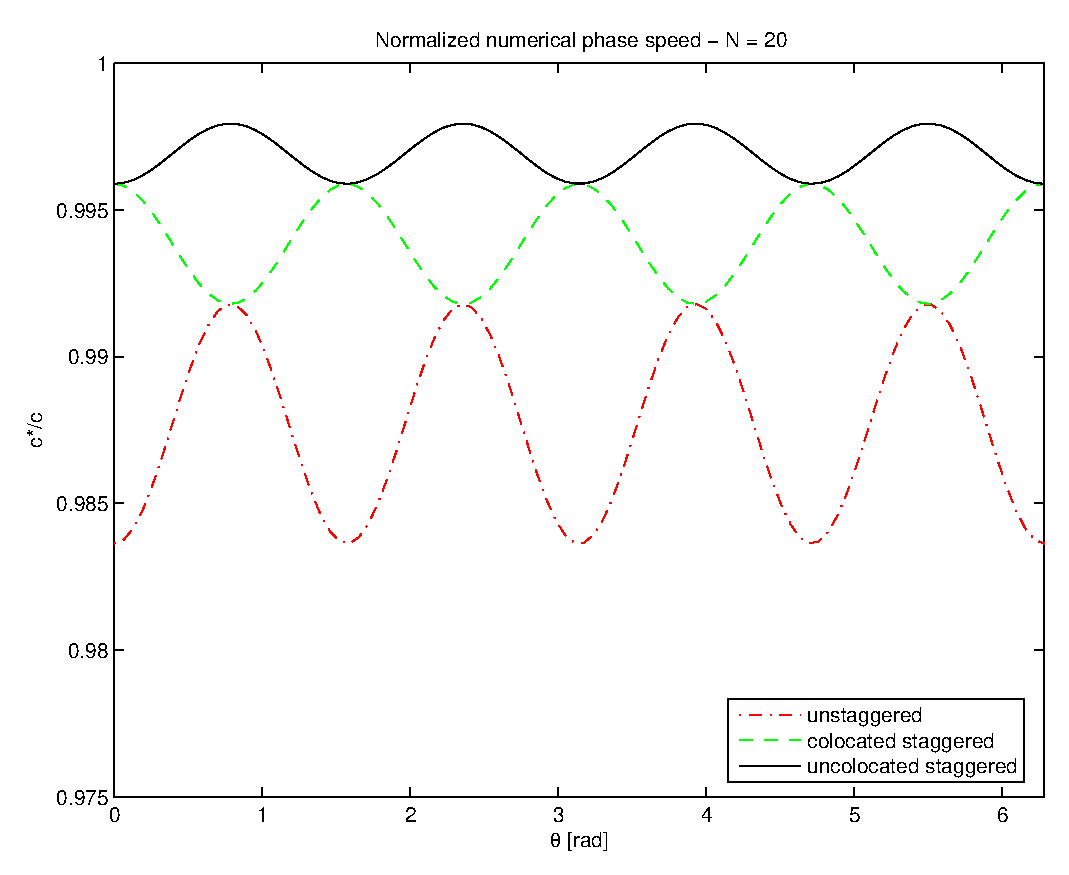
\includegraphics[height=8cm]{pics/liu_fourier_fig3}
  \end{center}
  \caption{Comparison of the normalized numerical phase speeds for
  Cartesian grids.}
  \label{fig:numerical_c}
\end{figure}  

From the \eqref{eqn:numerical_c2} we can note that the unstaggered
grid requires twice the number of points per wavelength in each
direction in order to have the same numerical phase speed as the
uncollocated staggered grid. In other words, for a given grid spacing
$\Delta s$, the error for the high frequency modes is greater than for
the low frequency modes, because we have less points per wavelength.

The error, defined as $1 - \frac{\Dual{c}}{c}$, is anisotropic
\ref{fig:numerical_c_polar}: greatest along the axes ($\theta = 0,
\pi/2, \pi, 3\pi/2$) and least along the diagonals ($\theta = \pi/4,
3\pi/4, 5\pi/4, 7\pi/4$) for both the unstaggered and uncollocated
staggered grids. The opposite is true for the collocated staggered
grid. Note that, even if a proper choice of the discretization scheme
in time can improve the overall dispersive error, it cannot completely
cancel it. This error depends only on the spatial discretization: the
medium ``grid'' is anisotropic itself.

\begin{figure}[htbp]
  \begin{center}
    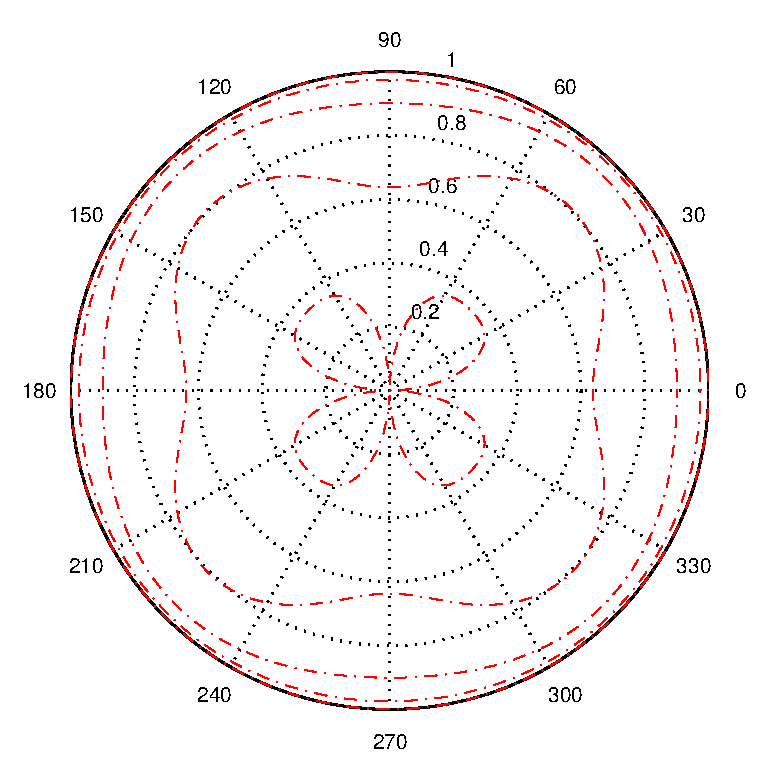
\includegraphics[width=3.5cm]{pics/liu_fourier_fig2a}
    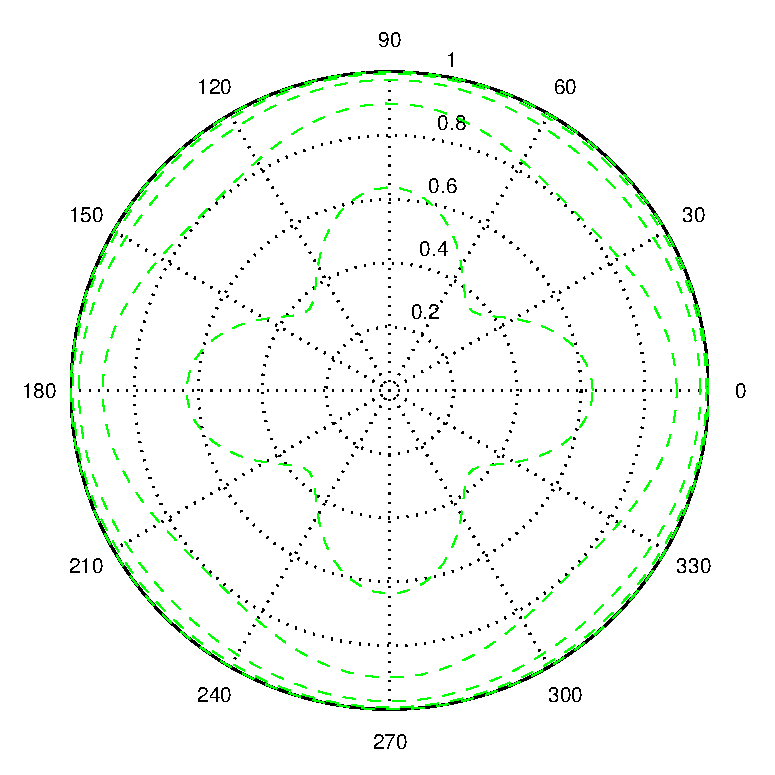
\includegraphics[width=3.5cm]{pics/liu_fourier_fig2b}
    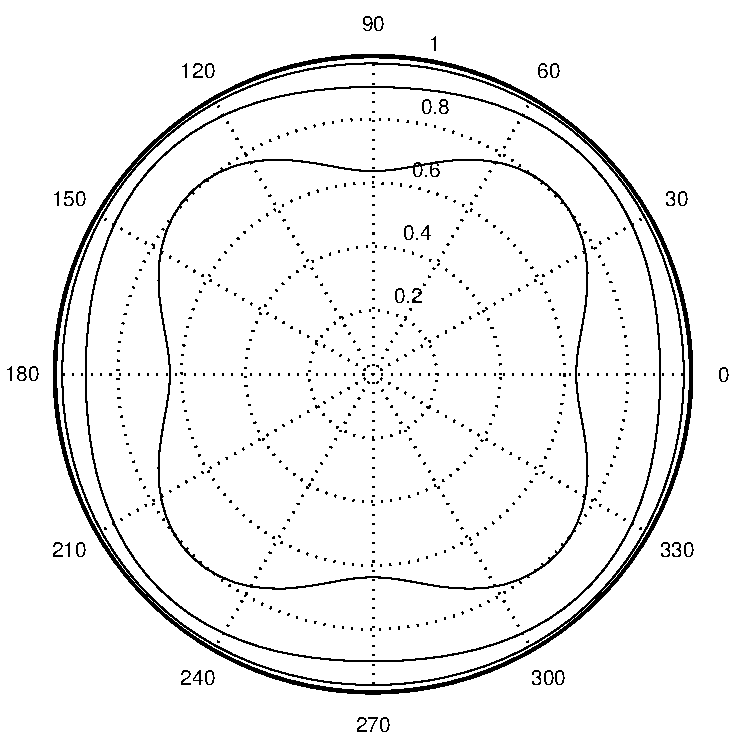
\includegraphics[width=3.5cm]{pics/liu_fourier_fig2c}
  \end{center}
  \caption{Polar diagrams of the normalized numerical phase speed for
  Cartesian grids and $N = 2, 4, 8, 16$: left, unstaggered grid,
  center, collocated staggered, right, uncollocated staggered.}
  \label{fig:numerical_c_polar}
\end{figure}  

We can define the \emph{isotropy error} as the difference between the
maximum and the minimum values of the normalized numerical phase speed
and we find that, for $N = 20$, it is $0.8\%$ on the unstaggered grid,
$0.4\%$ on the collocated staggered grid and $0.2\%$ on the uncollocated
staggered grid. In other words, to have the same isotropy error of
$0.1\%$ for the three schemes we need $N = 58, 41, 29$ grid points per
wavelength, respectively.

The dependence of the isotropy error on $N$ can be described expanding
in Taylor series the equations \eqref{eqn:numerical_c2}:
\begin{equation*}
  1-\frac{\Dual{c}}{c} = \begin{cases}
    \left( \frac{1}{2}  + \frac{1}{6} \cos 4\theta \right) \frac{\pi^2}{N^2} +
    \dotsb & \text{unstaggered} \\
    \left( \frac{1}{4}  - \frac{1}{12} \cos 4\theta \right) \frac{\pi^2}{N^2} +
    \dotsb & \text{collocated staggered} \\
    \left( \frac{1}{8}  + \frac{1}{24} \cos 4\theta \right) \frac{\pi^2}{N^2} +
    \dotsb & \text{uncollocated staggered}
    \end{cases}
\end{equation*}

The leading dispersive errors are proportional to $N^{-2}$,
i.e. doubling the coarseness of the grid reduces the dispersive error
by a factor 4.

From these considerations it should be clear that the uncollocated
staggered grid is the best choice:
\begin{itemize}
\item
  it is more computationally efficient
  \eqref{eqn:uncollocated_staggered};
\item
  it is 4 and 2 times more precise than the unstaggered and collocated
  staggered schemes, respectively, from a dispersive error point of
  view \eqref{eqn:numerical_c2}.
\end{itemize}

\subsubsection{Hexagonal grids}

The major deficiencies of conventional schemes come from their one
dimensional approach in which each spatial operator is approximated by
employing data only along one coordinate line. Since only a 5-point
Cartesian stencil is involved in each discretization, it is not
surprising that all three schemes described in the previous subsection
exhibit some anisotropy.

In this subsection we'll analyze a more efficient and accurate scheme,
not based on an orthogonal grid, but on a 7-point stencil on regular
hexagonal or triangular grid. This can also give a hint on the accuracy
of unstructured grids, which are topologically equivalent to this one.

We also use the information of the previous subsection, in which we
concluded that the uncollocated staggered scheme is the most efficient,
and we'll limit our study to the same scheme, but applied to the new
triangular grid.

\OKKIO{figure}

The equation \eqref{eqn:maxwell_2d} can be discretized as follows:
\begin{equation} \label{eqn:hexagonal_grid} \begin{split}
    d_t \Disc{D_z}{j,k}{} & = \frac{2 \left( \begin{aligned}
	\Disc{H_1}{j+1/4,k-\sqrt{3}/4}{} & -
	\Disc{H_1}{j-1/4,k+\sqrt{3}/4}{} + \\
	\Disc{H_2}{j+1/2,k}{} & - \Disc{H_2}{j-1/2,k}{} + \\
	\Disc{H_3}{j+1/4,k+\sqrt{3}/4}{} & -
	\Disc{H_3}{j-1/4,k-\sqrt{3}/4}{}
    \end{aligned} \right)}{3 \Delta s} \\
    d_t \Disc{B_1}{j+1/4,k-\sqrt{3}/4}{} & =
    \frac{\Disc{E_z}{j+1/2,k-\sqrt{3}/2}{} - \Disc{E_z}{j,k}{}}{\Delta s} \\
    d_t \Disc{B_2}{j+1/2,k}{} & = \frac{\Disc{E_z}{j+1,k}{} -
    \Disc{E_z}{j,k}{}}{\Delta s} \\
    d_t \Disc{B_3}{j+1/4,k+\sqrt{3}/4}{} & =
    \frac{\Disc{E_z}{j+1/2,k+\sqrt{3}/2}{} - \Disc{E_z}{j,k}{}}{\Delta s}
\end{split} \end{equation}

Again, the eigenvalues of the corresponding matrix $\Matrix{G}_s$ is
pure imaginary or zero, implying that this scheme is non-dissipative,
but dispersive.

Applying the Fourier analysis to the above equations, we obtain the
normalized numerical phase speed:
\begin{equation}
  \frac{\Dual{c}}{c} = \frac{\sqrt{8/3}}{\kappa \Delta s}\left[
  \sin^2 \frac{\xi}{2} + \sin^2 \left(\frac{\xi}{4} -
  \frac{\sqrt{3}\eta}{4}\right) + \sin^2 \left(\frac{\xi}{4} +
  \frac{\sqrt{3}\eta}{4}\right)\right]^{1/2}
\end{equation}
and the isotropy error:
\begin{equation}
  1-\frac{\Dual{c}}{c} = \frac{1}{8}\frac{\pi^2}{N^2} -
  \left(\frac{7}{1152} + \frac{1}{720} \cos 6\theta\right) \frac{\pi^4}{N^4} +
  \dotsb
\end{equation}

\begin{figure}[htbp]
  \begin{center}
    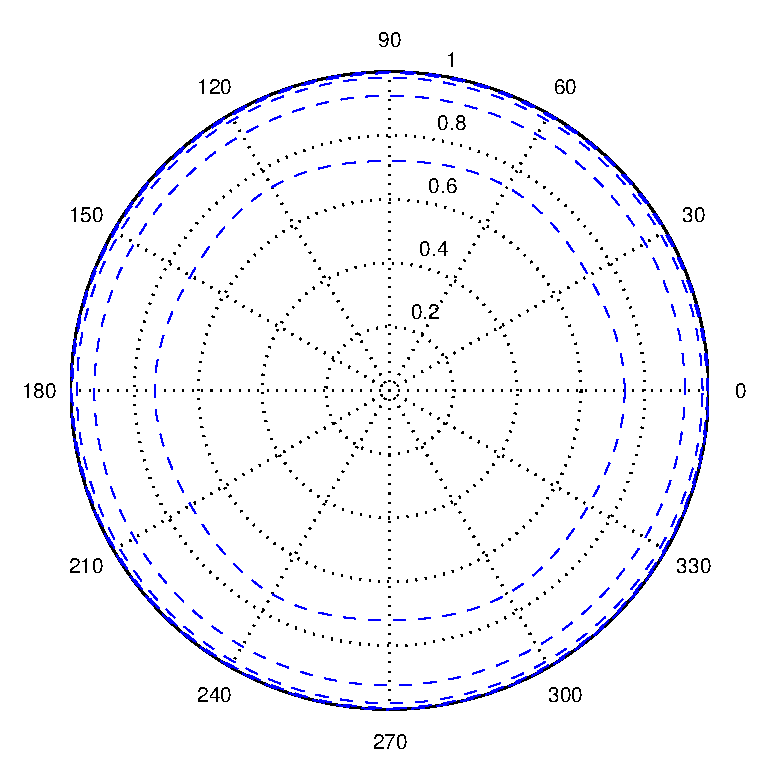
\includegraphics[height=8cm]{pics/liu_fourier_fig5b}
  \end{center}
  \caption{Polar diagram of the normalized numerical phase speed for
  hexagonal grids.}
  \label{fig:numerical_c_polar_hex}
\end{figure}  

\begin{figure}[htbp]
  \begin{center}
    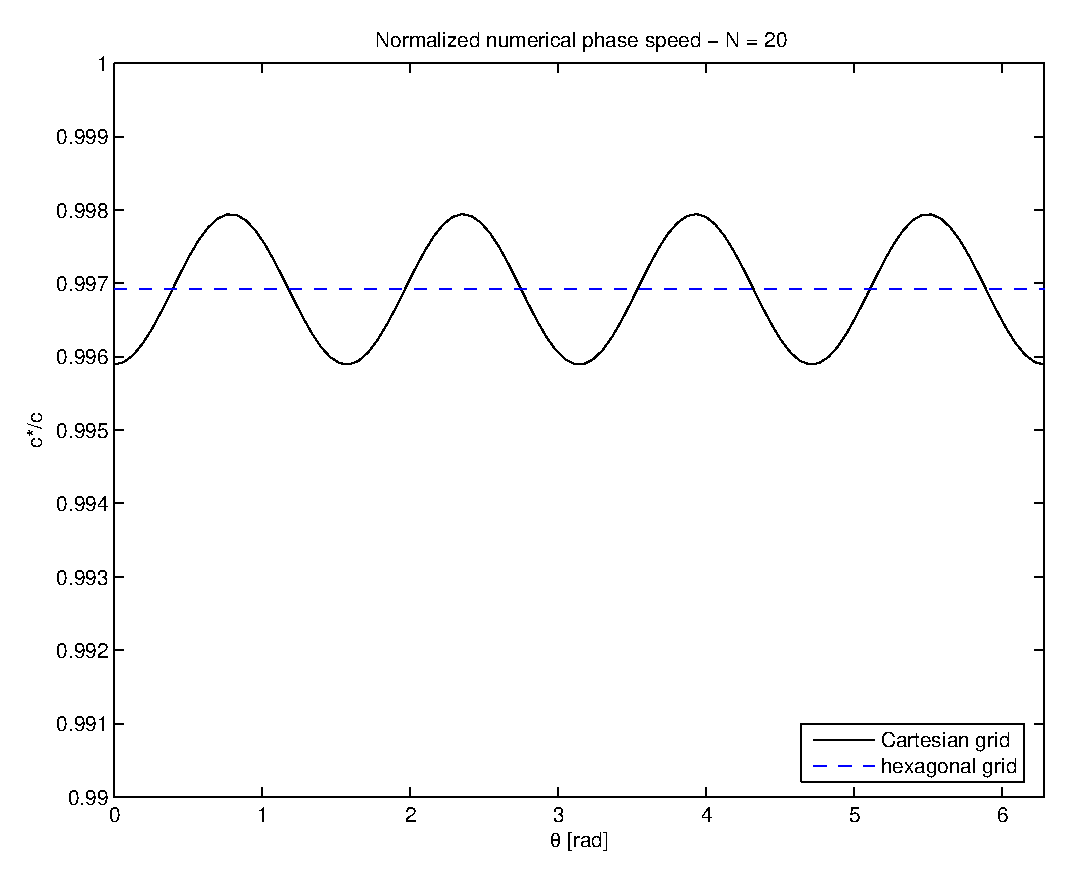
\includegraphics[height=8cm]{pics/liu_fourier_fig6}
  \end{center}
  \caption{Comparison of the normalized numerical phase speed for
  uncollocated staggered grids: Cartesian and hexagonal.}
  \label{fig:numerical_c_hex}
\end{figure}  

Even if the isotropy error is still leaded by a term proportional to
$N^{-2}$, it doesn't depend anymore on the direction of the wave
propagation \ref{fig:numerical_c_polar_hex}. Quite surprisingly, its
value is exactly the average of its Cartesian counterpart
\ref{fig:numerical_c_hex}.

The anisotropy appears in the fourth order term, which is two orders
of magnitude smaller than in the best Cartesian grid.

\subsection{Time discretization errors}

Time discretization, like spatial discretization, can also introduce
errors. However, these errors are only associated with dispersion and
dissipation and they are isotropic.

The equation \ref{eqn:maxwell_fourier} can be diagonalized, projecting
$\Vector{\mathcal{F}}$ on the eigenspace:
\begin{equation} \label{eqn:maxwell_fourier_eigen}
d_t f = \lambda f
\end{equation}
For a given time discretization, the amplification factor $\sigma$,
defined as the ratio of $f$ at two adjacent time levels $f = f^{n+1} /
f^n$ can be expressed as a function of $\lambda$\footnote{For example,
with a leapfrog time-stepping, \ref{eqn:maxwell_fourier_eigen} becomes:
$$
\Disc{f}{}{n+1} - \Disc{f}{}{n} = \deltat \lambda \Disc{f}{}{n+1/2} =
\frac{\deltat \lambda}{2} \left( \Disc{f}{}{n+1} + \Disc{f}{}{n}
\right) \Longrightarrow \Disc{f}{}{n+1} = \sigma \Disc{f}{}{n}
$$
where $\sigma = \frac{1+\frac{\lambda \deltat}{2}}{1-\frac{\lambda
    \deltat}{2}}$.
}.
Substituting the eigenvalues of $\Matrix{G}_s$ into $\sigma$, one
obtains the combined errors of spatial and time discretization and
\ref{eqn:maxwell_fourier} becomes:
$$
\Disc{\Vector{\mathcal{F}}}{}{n+1} = \Prod{\Matrix{G}}{\Disc{\Vector{\mathcal{F}}}{}{n}}
$$
$\Matrix{G}$ is called total amplification matrix. The eigenvalues of
$\Matrix{G}$ are the amplification factor $\sigma$. The modulus of
$\sigma$ determines the dissipative error and stability and the
argument determines the combined phase shift $\Dual{\phi} =
\Arg{\sigma}$.

Time integration of Maxwell's equations can be solved in many ways,
both explicitly and implicitly. While implicit schemes are usually
unconditionally stable, they require the solution of a linear
system. On the other hand, explicit schemes are conditionally stable
but they don't require any solution of a linear problem. The choice
between the two schemes must be done with the problem one wants to
solve in mind. For example, if one is interested in studying the
resonances of a particular device, it would be useful to look at a big
interval in time, so that all the transient waves can decay and only
the resonant ones survive: this would be best simulated with an
implicit scheme. An explicit scheme is best suited to study, for
example, the propagation of waves into a waveguide or the coupling
coefficient of a coupler: the time duration of the simulation is only
set by the physical length of the device, not by the accuracy
required, like in the resonance case.

We will only focus on explicit schemes. The most used ones are the
\emph{leapfrog} time-stepping and the \emph{Runge-Kutta} methods.
\begin{enumerate}
\item
  Leapfrog time-stepping: they are second-order and can be divided in:
  \begin{enumerate}
  \item
    staggered: if electric and magnetic fields are associated to two
    different time grids, staggered by half a time-step. So:
    \begin{equation} \label{eqn:lf1}
      \Disc{f}{}{n+1} = \Disc{f}{}{n} + \deltat d_t \Disc{f}{}{n+1/2}
    \end{equation}
    
    \OKKIO{disegno mio pag.406 liu fourier}
    
  \item
    unstaggered: if electric and magnetic fields are both associated
    to the same time grid:
    \begin{equation} \label{eqn:lf2}
      \Disc{f}{}{n+1} = \Disc{f}{}{n-1} + 2\deltat d_t \Disc{f}{}{n}
    \end{equation}
    
    \OKKIO{disegno mio pag.406 liu fourier}
    
  \end{enumerate}
\item
  Runge-Kutta methods: they use the fields computed at intermediate
  instants between two consecutive time steps, in order to increase
  accuracy:
  \begin{enumerate}
  \item
    third order:
    \begin{equation} \label{eqn:rk3} \begin{split}
      \Disc{f}{}{n+1/3} & = \Disc{f}{}{n} + \tfrac{1}{3} \deltat
      \Disc{d_t f}{}{n} \\
      \Disc{f}{}{n+2/3} & = \Disc{f}{}{n} + \tfrac{2}{3} \deltat
      \Disc{d_t f}{}{n+1/3} \\
      \Disc{f}{}{n+1} & = \Disc{f}{}{n} + \tfrac{1}{4} \deltat
      \left( 3\Disc{d_t f}{}{n+2/3} + \Disc{d_t f}{}{n} \right)
    \end{split} \end{equation}
  \item
    forth order:
    \begin{equation} \label{eqn:rk4} \begin{split}
      \Disc{\tilde{f}}{}{n+1/2} & = \Disc{f}{}{n} + \tfrac{1}{2} \deltat
      \Disc{d_t f}{}{n} \\
      \Disc{\hat{f}}{}{n+1/2} & = \Disc{f}{}{n} + \tfrac{1}{2} \deltat
      \Disc{d_t \tilde{f}}{}{n+1/2} \\
      \Disc{\bar{f}}{}{n+1} & = \Disc{f}{}{n} + \deltat \Disc{d_t \hat{f}}{}{n+1/2} \\
      \Disc{f}{}{n+1} & = \Disc{f}{}{n} + \tfrac{1}{6} \deltat
      \left( \Disc{d_t f}{}{n} + 2\Disc{d_t \tilde{f}}{}{n+1/2} +
      2\Disc{d_t \hat{f}}{}{n+1/2} + \Disc{d_t \bar{f}}{}{n+1} \right)
    \end{split} \end{equation}
  \end{enumerate}
\end{enumerate}

Using the equation \eqref{eqn:maxwell_fourier_eigen} and the above
equations, the amplification factors can be calculated. For example,
for the unstaggered leapfrog time-stepping \eqref{eqn:lf2} we can
write:
\begin{align}
  \Disc{f}{}{n+1} & = \Disc{f}{}{n} + \lambda \deltat
  \Disc{f}{}{n+1/2} \notag \\
  \Disc{f}{}{n-1} & = \Disc{f}{}{n} - \lambda \deltat
  \Disc{f}{}{n-1/2} \notag \\
  \intertext{Summing each member:}
  \Disc{f}{}{n+1} + \Disc{f}{}{n-1} & = 2\Disc{f}{}{n} + \lambda
  \deltat (\Disc{f}{}{n+1/2} + \Disc{f}{}{n-1/2}) \notag \\
  & = \left[ 2 + \left( \lambda \deltat \right)^2 \right]
  \Disc{f}{}{n} \notag \\
  \intertext{therefore:}
  \sigma + \frac{1}{\sigma} & = 2 + \left( \lambda \deltat \right)^2
  \notag \\
  \sigma_{1,2} & = \lambda \deltat \pm \sqrt{\left( \lambda \deltat
  \right) + 1} \notag
\end{align}

The same procedure can be applied to the other time integration
schemes, obtaining:
\begin{equation} \label{eqn:sigma}
  \sigma = \begin{cases}
    1+\frac{1}{2} \left( \lambda \deltat \right)^2 \pm \sqrt{\left[ 1
    + \frac{1}{2} \left( \lambda \deltat \right)^2 \right]^2 - 1} &
    \text{for \eqref{eqn:lf1}} \\
    \left( \lambda \deltat \right) \pm \sqrt{\left( \lambda \deltat \right)^2 + 1} &
    \text{for \eqref{eqn:lf2}} \\
    1+ \lambda \deltat + \frac{1}{2} \left( \lambda \deltat \right)^2
    + \frac{1}{6} \left( \lambda \deltat \right)^3 & \text{for \eqref{eqn:rk3}} \\
    1+ \lambda \deltat + \frac{1}{2} \left( \lambda \deltat \right)^2
    + \frac{1}{6} \left( \lambda \deltat \right)^3 + \frac{1}{24}
    \left( \lambda \deltat \right)^4 & \text{for \eqref{eqn:rk4}}
  \end{cases}
\end{equation}

Stability is obtained if $\Abs{\sigma} < 1$. In the hypothesis of
$\lambda = \imath \lambda_I$, purely imaginary, for the staggered
leapfrog algorithm: $\Abs{\sigma} < 1 \iff \Abs{1 - \frac{1}{2}
\lambda^2 \deltat^2} < 1 \iff \lambda \deltat \in \left[ -2, 2 \right]
- \left\{ 0 \right\}$. The method is conditionally stable. For the
unstaggered leapfrog algorithm: $\Abs{\sigma}^2 = \left( \lambda_I
\deltat \right)^2 + \left( 1 - \left( \lambda_I \deltat \right)^2
\right) = 1 \quad \forall \deltat$: this method is unconditionally
unstable.

Both the Runge-Kutta methods are conditionally stable. For an imaginary
$\lambda$, the two leapfrog time-stepping schemes are non-dissipative
but the Runge-Kutta methods are. They are all dispersive.

\subsection{Space and Time discretization}

From the above considerations, one could think that the forth order
Runge-Kutta method is the most accurate time integration method for
electromagnetic problems. This is correct only if we don't consider
the spatial discretization: errors can cancel out. Indeed, for central
difference spatial discretization, leapfrog time-stepping is more
accurate than Runge-Kutta.

The staggered leapfrog time-stepping in time combined with a staggered
central difference in space is non-dissipative and the least
dispersive: applied to Cartesian grid, it is called \emph{Yee scheme}
\cite{yee_boh}.

\section{feprop -- my notes}

\OKKIO{cercare in tutti gli articoli di tonti, bossavit, codecasa
  considerazioni sulle griglie di Vorono\"i, Poincar\'e e
  baricentriche}

Material matrices are also called \emph{mass matrices} in Finite
Elements context and \emph{discrete Hodge operators} in differential
geometry. Their shape affects the stability of time- and frequency-
domain \cite{schuhmann_whitney} \cite{schuhmann_stability}.

\subsection{Vorono\"i 2D} \label{sec:voronoi}

Given a primal triangular mesh, the Vorono\"i dual mesh is built
connecting the spherocenters of the primal volumes, i.e. the centers
of the spheres that contain each primal volume. Some properties hold:
\begin{itemize}
\item
  dual edges are orthogonal to primal faces;
\item
  primal edges are orthogonal to dual faces;
\item
  dual volumes are the loci of nearest points to the corresponding
  primal point.
\end{itemize}

These properties represent, as we'll see later, advantages in modeling
Maxwell's equations, but they are tough geometrical
constrains. Indeed, not all the primal meshes have a valid Vorono\"i
dual mesh, in the sense that the Vorono\"i mes is itself a proper mesh
\OKKIO{reference alle proprieta' di una mesh -- che ricopra lo spazio,
non si sovrapponga, etc.}. Consider, for example, figure
\ref{fig:voronoi_bad}: for the sake of simplicity, a 2D triangular
mesh. Its Vorono\"i dual mesh is obtained connecting the circumcenters
of the primal triangles. We can see that, in this case, the dual faces
overlaps and do not satisfy one of the properties of \emph{good
mesh}. Meshes that have a proper Vorono\"i dual mesh are called
\emph{Delaunay} meshes. One very simple example of a Delaunay mesh is
a mesh made of triangles whose angles are all less that $90\degrees$:
in fact, for this kind of triangles, the circumcenter lies always
inside the corresponding triangle and no pathological situations
arise. Indeed, the possibility that, even for a Delaunay mesh, the
circumcenter of a triangle lies outside the corresponding triangle,
can represent a problem in electromagnetic simulations and should be
avoided. For this reason, sometimes more stringent geometrical
constrains on primal meshes are imposed, to ensure that this doesn't
happen. \OKKIO{reference a triangle e easymesh}.

Consider a Delaunay primal mesh and its Vorono\"i dual mesh: let's
limit to the 2D case, because the extension to the 3D case is
straightforward, and consider the Maxwell's equations for the TE
polarization\footnote{the TM case can be studied using the duality
  theorem}.

Let:
\begin{align} \label{eqn:dof_voronoi}
e_i & = \DotProd{\E}{\Versor{p}_i} \ell_i \\
h_i & = \DotProd{\H}{\Versor{s}_i} \Dual{\ell}_i \\
b_i & = \DotProd{\B}{\Versor{s}_i} A_i \\
d_i & = \DotProd{\D}{\Versor{p}_i} \Dual{A}_i
\end{align}
where $\Versor{p}_i$ ($\Versor{s}_i$) is the primal (dual) edge
versor. Note that $\Versor{p}_i$ is orthogonal to $\Versor{s}_i$.

Maxwell's equations read:
\begin{equation} \label{eqn:maxwell_voronoi} \begin{cases}
    \Disc{b_i}{}{n+1/2} & = \Disc{b_i}{}{n-1/2} - \deltat \sum_{j \in
    N_{A_i}} \Disc{e_j}{}{n} \\
    \Disc{d_i}{}{n+1} & = \Disc{d_i}{}{n-1} + \deltat \sum_{j \in
    N_{\Dual{A}_i}} \Disc{h_j}{}{n+1/2}
  \end{cases} \end{equation}
where $N_{A_i}$ is the set of the indices that identifies the border
edges of the primal face $A_i$:
\begin{equation*}
  N_{A_i} = \left\{ j\ :\ \ell_j \in \partial A_i \right\}
\end{equation*}
where $\partial A$ denotes the boundary of the face $A$, and
$N_{\Dual{A}_i}$ is the set of the indices that identifies the border
edges of the dual face $\Dual{A}_i$:
\begin{equation*}
  N_{\Dual{A}_i} = \left\{ j\ :\ \Dual{\ell}_j \in \partial \Dual{A}_i
  \right\}
\end{equation*}

Thank to the properties of Vorono\"i meshes, the constitutive
equations are straightforward. From \eqref{eqn:dof_voronoi}, consider
the $i^{th}$ primal face, and the corresponding $i^{th}$ dual edge; we
can write:
\begin{equation} \label{eqn:constitutive_voronoi_magnetic}
  h_i = \frac{\Dual{\ell}_i}{A_i \mu_i} b_i
\end{equation}
where $\mu_i$ is the magnetic permeability associated to the primal
face $A_i$. The other constitutive equation, for the $i^{th}$ primal
edge and the $i^{th}$ dual face, reads:
\begin{equation} \label{eqn:constitutive_voronoi_electric}
  e_i = \frac{\ell_i}{\Dual{A}_i \epsilon_i} d_i
\end{equation}
where $\epsilon_i$ is the electric permeability associated to the dual
face $\Dual{A}_i$.

\OKKIO{anisotropia}

\OKKIO{distinguere tra faccia e area della faccia, lato e misura del
  lato, etc.}

\OKKIO{spiegare come $\epsilon$ e $\mu$ sono associati agli elementi
  geometrici}

Note that the value of $h_i$ ($e_i$) only depends on the value of
$b_i$ ($d_i$) on the corresponding (dual) face. Writing them in matrix
form, we have:
\begin{align*}
  \Array{h} & = \Prod{\Matrix{M}_\mu}{\Array{b}} \\
  \Array{e} & = \Prod{\Matrix{M}_\epsilon}{\Array{d}}
\end{align*}
where $\Array{h}$ and $\Array{b}$ are the array of all the $h_i$ and
$b_i$ in \eqref{eqn:maxwell_voronoi} and $\Matrix{M}_\mu$ and
$\Matrix{M}_\mu$ are diagonal matrices whose dimensions are the number
of dual and primal faces, respectively.

\subsection{Poincar\'e 2D} \label{sec:poicare}

Given a primal triangular mesh, the Poincar\'e dual mesh is built
connecting the barycenters of the primal volumes. Comparing to the
Vorono\"i dual mesh, we can note:
\begin{enumerate}
\item
  the dual points are always inside the primal volumes: this makes the
  scheme more stable in the time-domain;
\item
  the dual edges are not orthogonal to the primal faces and the primal
  edges are not orthogonal to the dual faces: this makes the
  constitutive relations more complicated to implement.
\end{enumerate}

Consider a 2D triangular primal mesh and let's limit to the study of
the TE polarization\footnote{for the TM polarization, the duality
  theorem can be applied \OKKIO{citare il duality theorem}; the
  extension to the 3D case is straightforward, too.}: let $E_z$ be
associated to the nodes of the primal grid and $\H_t$ to the edges of
the dual grid.

\OKKIO{figura Poincar\'e dual mesh}

Let:
\begin{align} \label{eqn:dof_poincare}
e_i & = \DotProd{\E}{\Versor{p}_i} \ell_i \\
h_i & = \DotProd{\H}{\Versor{s}_i} \Dual{\ell}_i \\
b_i & = \DotProd{\B}{\Versor{n}_{p_i}} A_i \\
d_i & = \DotProd{\D}{\Versor{n}_{s_i}} \Dual{A}_i
\end{align}
where $\Versor{p}_i$ ($\Versor{s}_i$) is the primal (dual) edge
versor and $\Versor{n}_{p_i}$ ($\Versor{n}_{s_i}$) is the versor
orthogonal to the primal (dual) face. As noted before,
$\Versor{n}_{p_i}$ is not parallel to $\Versor{s}_i$ and
$\Versor{n}_{s_i}$ is not parallel to $\Versor{p}_i$ as in
Vorono\"i dual grids.

Maxwell's equations, being topological relations, are the same as in
the Vorono\"i meshes:
\begin{equation} \label{eqn:maxwell_poincare} \begin{cases}
    \Disc{b_i}{}{n+1/2} & = \Disc{b_i}{}{n-1/2} - \deltat \sum_{j \in
    N_{A_i}} \Disc{e_j}{}{n} \\
    \Disc{d_i}{}{n+1} & = \Disc{d_i}{}{n-1} + \deltat \sum_{j \in
    N_{\Dual{A}_i}} \Disc{h_j}{}{n+1/2}
  \end{cases} \end{equation}
where $N_{A_i}$ is the set of the indices that identifies the border
edges of the primal face $A_i$:
\begin{equation*}
  N_{A_i} = \left\{ j\ :\ \ell_j \in \partial A_i \right\}
\end{equation*}
where $\partial A$ denotes the boundary of the face $A$, and
$N_{\Dual{A}_i}$ is the set of the indices that identifies the border
edges of the dual face $\Dual{A}_i$:
\begin{equation*}
  N_{\Dual{A}_i} = \left\{ j\ :\ \Dual{\ell}_j \in \partial \Dual{A}_i
  \right\}
\end{equation*}

Constitutive equations are more complicated because $\H_t \nparallel
\B_t$. For the electric one, the same relation as in the Vorono\"i
case holds \eqref{eqn:constitutive_voronoi_electric}. For the magnetic
case, recall that we have to write:
\begin{equation*}
  \Array{h} = \Prod{\Matrix{M}_\mu}{\Array{b}}
\end{equation*}
where $\Array{h}$ and $\Array{b}$ are the array of all the $h_i$ and
$b_i$ in \eqref{eqn:maxwell_poincare} and $\Matrix{M}_\mu$ is a square
matrix whose dimension is the number of dual edges\footnote{or primal
  faces, that is the same, if the mesh is not pathological
  \OKKIO{spiegare meglio}}.

This can be done in three steps.
\begin{enumerate}
\item
  Write $\B_j$ as a linear combination of $b_i$ and $b_j$.\\
  \newline
  \OKKIO{figura}
  Consider the $i^{th}$ primal edge and let $j$ identify all the other
  primal edges appended\footnote{i.e., having a node in common} to
  it. Now let:
  \begin{equation*} \begin{aligned}
      \Vector{N}_{p_i} & = \Versor{n}_{p_i} A_i \\
      \Vector{N}_{p_j} & = \Versor{n}_{p_j} A_j
  \end{aligned} \end{equation*}
  Flux conservation requires that:
  \begin{equation*} \left\{ \begin{aligned}
      \DotProd{\B_j}{\Vector{N}_{p_i}} & =
      \DotProd{\B}{\Vector{N}_{p_i}} & = b_i \\
      \DotProd{\B_j}{\Vector{N}_{p_j}} & =
      \DotProd{\B}{\Vector{N}_{p_j}} & = b_j
  \end{aligned} \right. \end{equation*}
  The right-hand sides are knows from the Faraday equation (the first
  in \eqref{eqn:maxwell_poincare}), so we can calculate $\B_j$:
  \begin{equation*}
    \B_j = \Prod{\Matrix{N}^{-1}}{\begin{bmatrix} b_i \\ b_j \end{bmatrix}}
    \qquad \text{where} \qquad \Matrix{N} = \begin{bmatrix} N^x_{p_i}
    & N^y_{p_i} \\ N^x_{p_j} & N^y_{p_j} \end{bmatrix}
  \end{equation*}
\item
  Write $\B$ as a linear combination of $\B_j$.\\
  \newline
  \begin{equation*}
    \B_i = \frac{1}{W} \sum_j w_j \B_j
  \end{equation*}
  where $W = \sum_j w_j$ and $w_j = \Norm{\DotProd{\Versor{z}}{\left(
  \CrossProd{\Vector{N}_{p_i}}{\Vector{N}_{p_j}} \right)}}$,
  i.e. twice the area of the triangle identified by the edges $i$ and
  $j$.
\item
  Compute $\H$ from the constitutive relation $\H = \mu^{-1} \B$ and
  then $h_i$, from \eqref{eqn:dof_poincare}.\\
  \newline
  \begin{equation} \label{eqn:constitutive_magnetic_poincare} \begin{split}
    h_i & = \DotProd{\H}{\Versor{s}_i} \Dual{\ell}_i \\
    & = H_x \Dual{\ell}_i \cos\beta + H_y \Dual{\ell}_i \sin\beta \\
    & = \mu_x^{-1} B_x \Dual{\ell}_i \cos\beta +
    \mu_y^{-1} B_y \Dual{\ell}_i \sin\beta \\
    & = \frac{1}{W} \sum_j w_j \left[ \mu_x^{-1} B_x \Dual{\ell}_i
    \cos\beta + \mu_y^{-1} B_y \Dual{\ell}_i
    \sin\beta \right] \\
    & = \frac{1}{W} \sum_j w_j \left[ \mu_x^{-1} \Dual{\ell}_i
    \cos\beta \left( k_{11} b_i + k_{12} b_j \right) +
    \mu_y^{-1} \Dual{\ell}_i \sin\beta \left( k_{21} b_i +
    k_{22} b_j \right) \right] \\
    & = \frac{\Dual{\ell}_i}{W} \sum_j w_j \left[ \left( \mu_x^{-1} k_{11}
    \cos\beta + \mu_y^{-1} k_{21} \sin\beta
    \right) b_i + \left( \mu_y^{-1} k_{12}
    \cos\beta + \mu_y^{-1} k_{22} \sin\beta
    \right) b_j \right]
  \end{split} \end{equation}
  where $\beta$ is the angle between the dual edge $\Dual{\ell}_i$ and
  the $x$-axis and $\Matrix{K} = \bigl[ \begin{smallmatrix}
  k_{11}&k_{12}\\k_{21}&k_{22} \end{smallmatrix} \bigr] =
  \Matrix{N}^{-1}$.
  
  In matricial form:
  \begin{equation*}
    \Array{h} = \Prod{\Matrix{M}_\mu}{\Array{b}}
  \end{equation*}
  where
  \begin{equation} \label{eqn:constitutive_poincare}
    \Matrix{M}_\mu = \begin{bmatrix}
      {\Matrix{M}_\mu}_{ij}
    \end{bmatrix} = \begin{cases}
      \frac{\Dual{\ell}}{W} \sum_j w_j 
    \left( \mu_x^{-1} k_{11} \cos\beta + \mu_y^{-1} k_{21} \sin\beta
    \right) & \text{for $i = j$} \\
      \frac{\Dual{\ell}}{W} w_j 
    \left( \mu_x^{-1} k_{12} \cos\beta + \mu_y^{-1} k_{22} \sin\beta
    \right) & \text{for $i \neq j$} \\
    \end{cases}
  \end{equation}
\end{enumerate}

It is worth noting that:
\begin{itemize}
\item
  these three steps are fully explicit, i.e. we
  don't ever need to solve a linear system to compute the unknowns we
  need;
\item
  the final matrix $\Matrix{M}_\mu$ is not diagonal, as
  explicitly stated in \eqref{eqn:constitutive_poincare}: one may
  think this could be a problem in the frequency domain, but we'll
  show that this is not the case\footnote{\OKKIO{la matriciona si
  ottiene senza invertire niente! -- mettere riferimento alla
  formula}};
\item
  \eqref{eqn:constitutive_magnetic_poincare} is valid also for
  anisotropic materials: just use a tensor $\mu = \left[
  \begin{smallmatrix} \mu_{xx} & \mu_{xy} \\ \mu_{yx} & \mu_{yy}
  \end{smallmatrix} \right]$. Note also that dealing with an
  anisotropic material is equivalent in introducing a local change of
  metric. In fact, for the simple case of a coordinate system oriented
  with the crystallographic axis of the anisotropic
  material\footnote{If not, a simple rotation of the reference axis
  can bring us to this condition}:
  \begin{equation*} \begin{split}
    h_i & = \Prod{\left( \mu^{-1} \B \right)}{\Versor{s}_i} \Dual{\ell}_i \\
        & = \left( \mu_x^{-1} {s_i}_x B_x + \mu_y^{-1} {s_i}_y B_y \right) \Dual{\ell}_i \\
        & = \Prod{\B}{\Vector{s}'_i} \Dual{\ell}_i
  \end{split} \end{equation*}
  where $\Vector{s}'_i = \left( \mu_x^{-1} {s_i}_x, \mu_y^{-1}
  {s_i}_y \right)$. The metric, as said before, is needed when dealing
  with the material equations.
\end{itemize}

\subsection{Barycentric 2D} \label{sec:barycentric}

Given a triangular primal mesh, its barycentric dual is made of:
\begin{itemize}
\item
  dual points that are the barycenters of the primal volumes;
\item
  dual edges that are piece-lines made by two straight lines whose
  contact point is the barycenter of the corresponding primal face,
  and connect the dual points;
\item
  dual surfaces having as a border the dual lines surrounding the
  corresponding primal edge.
\end{itemize}

\OKKIO{figure: 2D, 2D estruso e 3D}

Since primal and dual meshes are not orthogonal, as in the Poincar\'e
mesh, the constitutive equation requires some math to be worked
out. The advantage of this mesh is its superior stability and the
possibility to use any kind of triangular grid, not only a Delaunay
one.

Consider a 2D TE case: the degrees of freedom are as in
\eqref{eqn:dof_poincare}. Consider the figure \OKKIO{figure 11 di
  marrone computational}, and divide the primal volume, as shown, in 6
\emph{micro-cells}. For each micro-cell, we can write:
\begin{align}
  \begin{bmatrix} \Phi_{1U''} \\ \Phi_{2U'} \end{bmatrix} = \Prod{
  \begin{bmatrix} S_{1U_x''} & S_{1U_y''} \\ S_{2U_y'} & S_{2U_y'}
  \end{bmatrix}}{
  \begin{bmatrix} B_x \\ B_y \end{bmatrix}}
\end{align}
where $\Phi$ is the magnetic flux through the primal face $S$, and
$\Vector{S}_{1U}$ is the vector normal to the primal face $1U$, whose
modulus is equal the area of the face. Something similar holds for the
$\H$ field:
\begin{align}
  \begin{bmatrix} F_{1U''} \\ F_{2U'} \end{bmatrix} = \Prod{
  \begin{bmatrix} \Dual{\ell}_{1U_x''} & \Dual{\ell}_{1U_y''} \\
    \Dual{\ell}_{2U_y'} & \Dual{\ell}_{2U_y'} \end{bmatrix}}{
  \begin{bmatrix} H_x \\ H_y \end{bmatrix}}
\end{align}
where $F$ is the circuitation of $\H$ along the dual line
$\Dual{\ell}$.

We can combine the two equations and the material equation $\B = \mu
\H$, to obtain:
\begin{align} \label{eqn:constitutive_barycentric_microcell}
  \begin{bmatrix} \Phi_{1U''} \\ \Phi_{2U'} \end{bmatrix} = \Prod{
  \underbrace{
  \begin{bmatrix} S_{1U_x''} & S_{1U_y''} \\ S_{2U_y'} & S_{2U_y'}
  \end{bmatrix}
  \mu
  \begin{bmatrix} \Dual{\ell}_{1U_x''} & \Dual{\ell}_{1U_y''} \\
    \Dual{\ell}_{2U_y'} & \Dual{\ell}_{2U_y'} \end{bmatrix}^{-1}
  }_{\Matrix{M}_\mu}}{
  \begin{bmatrix} F_{1U''} \\ F_{2U'} \end{bmatrix}}
\end{align}
This constitutive equation holds for the each micro-cell considered. We
can write 6 equations like this, one for each micro-cell in which the
primal volume is divided. Finally, we connect each other by continuity
condition, to get the final constitutive equation. For the continuity
of the $\H$ tangential component, we have:
\begin{align}
  F_{1U}' & = F_{1L}' & F_{1U}'' & = F_{1L}'' \\
  F_{2U}' & = F_{2L}' & F_{2U}'' & = F_{2L}'' \\
  F_{3U}' & = F_{3L}' & F_{3U}'' & = F_{3L}''
\end{align}
For the additivity of the flux of $\B$, i.e. the conservation of the
normal component of $\B$, we have:
\begin{align}
  \Phi_{1U}' + \Phi_{1U}' & = \Phi_{1}' & \Phi_{1U}'' + \Phi_{1U}'' & = \Phi_{1}'' \\
  \Phi_{2U}' + \Phi_{2U}' & = \Phi_{2}' & \Phi_{2U}'' + \Phi_{2U}'' & = \Phi_{2}'' \\
  \Phi_{3U}' + \Phi_{3U}' & = \Phi_{3}' & \Phi_{3U}'' + \Phi_{3U}'' & = \Phi_{3}''
\end{align}
Again, imposing the continuity of the $\H$ field:
\begin{align}
  F_1' & = F_1'' \\
  F_2' & = F_2'' \\
  F_3' & = F_3''
\end{align}
and the additivity of the flux of $\B$:
\begin{align}
  \Phi_1' + \Phi_1'' & = \Phi_1 \\
  \Phi_2' + \Phi_2'' & = \Phi_2 \\
  \Phi_3' + \Phi_3'' & = \Phi_3
\end{align}
This leads us to write the constitutive equation for the primal cell:
\begin{equation} \label{eqn:constitutive_barycentric}
  \begin{bmatrix} \Phi_1 \\ \Phi_2 \\ \Phi_3 \end{bmatrix} = \Prod{
  \underbrace{
    \begin{bmatrix}
      {M_\mu^a}_{11} & {M_\mu^a}_{12} & 0 \\
      {M_\mu^a}_{21} & {M_\mu^a}_{22} & 0 \\
      0 & 0 & 0 \\
    \end{bmatrix} +
    \begin{bmatrix}
      0 & 0 & 0 \\
      0 & {M_\mu^b}_{11} & {M_\mu^b}_{12} \\
      0 & {M_\mu^b}_{21} & {M_\mu^b}_{22}
    \end{bmatrix} +
    \begin{bmatrix}
      {M_\mu^c}_{22} & 0 & {M_\mu^c}_{21} \\
      0 & 0 & 0 \\
      {M_\mu^c}_{12} & 0 & {M_\mu^c}_{11}
    \end{bmatrix}
    }_{\Matrix{M}_\mu}}{
  \begin{bmatrix} F_1 \\ F_2 \\ F_3 \end{bmatrix}}
\end{equation}

On a perfectly dual way, the electric constitutive equation can be
written.

Note that anisotropy is readily implemented considering a tensor $\mu
= \left[ \begin{smallmatrix} \mu_{xx} & \mu_{xy} \\ \mu_{yx} &
  \mu_{yy} \end{smallmatrix} \right]$ in
\eqref{eqn:constitutive_barycentric_microcell}.

\subsection{Two dimensional extrude grids}

It is obtained by extrusion along the third dimension of a
two-dimensional grid. Good for planar structures.

\subsection{Particular material equations} \label{sec:particular_material_equations}

In the previous subsections the conventional material equations have
been discretized. We'll show now how more complex materials can be
modeled with the present method.

\subsubsection{Anisotropic materials}

\OKKIO{mettere qui i materiali anisotropi -- local change of metric}

\subsubsection{Ohm losses}

Equation \eqref{eqn:maxwell_time_domain} is missing the description of
the Ohm losses. It can be easily included, as follows:
\begin{equation*} \begin{cases}
  \Prod{\Transpose{\Matrix{R}}}{\Array{h}} = \partial_t \Array{d} + \Array{j} + \Matrix{\sigma_e} \Array{e} \\
  \Prod{\Matrix{R}}{\Array{e}} = -\partial_t \Array{b} + \Array{m} - \Matrix{\sigma_m} \Array{h}
\end{cases} \end{equation*}
According to the association of the degrees of freedom to the
geometrical elements of the mesh, supposing that the electric field
associated to a primal edge and the conductibility are uniform over the
corresponding dual face, we can easily build the matrices
$\Matrix{\sigma_e}$ and $\Matrix{\sigma_m}$ as the material matrices,
with the procedures described above, depending on the particular dual
grid chosen. The only problem arises in the time domain: in fact, the
matrix/operator $\Matrix{\sigma_e}$ ($\Matrix{\sigma_m}$) must link a
physical quantity defined on the primal instants (the electric field)
with one defined on the dual instants (the magnetic field). Hence, it
must be estimated by some means of time approximation. The easiest way
to do it, which keeps the algorithm stable, is to approximate the
electric field at the time-step $n+1/2$ as the mean value of the
instants before and after it:
\begin{equation*}
  \Disc{\Array{e}}{}{n+1/2} \simeq \frac{\Disc{\Array{e}}{}{n} + \Disc{\Array{e}}{}{n+1}}{2}
\end{equation*}
With this choice, \eqref{eqn:maxwell_time_domain} only involve fields
defined in the \emph{proper} time instants, and the algorithm is
stable (and second order accurate in the time derivative).

The same reasoning holds for the magnetic conductivity
$\Matrix{\sigma_m}$\footnote{Even if the magnetic conductivity can
  appear a useless physical quantity, it is not, because it is used in
  the modelling of PML losses}.

It should be clear that this problem only arises in the
time-domain. In the frequency domain, the easiest way to deal with Ohm
losses is to accept a complex value for the electric and magnetic
permeabilities. In formulas:
\begin{equation*}
    \begin{cases}
      \Rot{\H} = -\imath \omega \epsilon \E + \sigma_e \E \\
      \Rot{\E} = \imath \omega \mu \H + \sigma_m \H \\
    \end{cases}
    \Longrightarrow
    \begin{cases}
      \Rot{\H} = -\imath \omega \bar{\epsilon} \E \\
      \Rot{\E} = \imath \omega \bar{\mu} \H \\
    \end{cases}
\end{equation*}
where $\bar{\epsilon} = \epsilon + \imath \frac{\sigma_e}{\omega}$ and
$\bar{\mu} = \mu + \imath \frac{\sigma_m}{\omega}$. Obviously, also
the material matrices $\Matrix{M}_\epsilon$ and $\Matrix{M}_\mu$ will
be complex.

As a first approximation, we can disregard this problem, even in the
time-domain, and write: \OKKIO{controllare!!!}
\begin{equation*} \begin{cases}
    \frac{\Disc{\Array{b}}{}{n+1} - \Disc{\Array{b}}{}{n}}{\deltat} = -
    \Prod{\Matrix{R}}{\Disc{\Array{e}}{}{n+1/2}} -
    \Prod{\Matrix{\Omega}_{MN}}{\Disc{\Array{h}}{}{n-1}} \\
    \frac{\Disc{\Array{d}}{}{n+1/2} - \Disc{\Array{d}}{}{n-1/2}}{\deltat} = 
    \Prod{\Transpose{\Matrix{R}}}{\Disc{\Array{e}}{}{n+1/2}} -
    \Prod{\Matrix{\Omega}_{EN}}{\Disc{\Array{e}}{}{n-1/2}}
\end{cases} \end{equation*}
For later convenience, let $\Matrix{P}_m =
\Prod{\Matrix{M}_\mu}{\Matrix{\Omega}_{MN}}$ and $\Matrix{P}_e =
\Prod{\Matrix{M}_\epsilon}{\Matrix{\Omega}_{EN}}$.

$\Matrix{\Omega}_{MN}$ and $\Matrix{\Omega}_{EN}$ can be built
following the same procedure used for the material matrices.

\subsubsection{U-PML}

PML are used to model infinite materials, i.e. to model the radiation
of light as if the boundaries of the computational domain were at
infinite distance from the source. There are mainly two formulations
to model the PMLs:
\begin{description}
\item[coordinate stretching]: in which a local change of metric is
  introduced where attenuation is needed, so that any plane wave
  impinging at the interface undergoes no reflection, but
  exponentially decays at zero;
\item[Uniaxial PML]: in which an anisotropic lossy material, but fully
  Maxwellian, is defined, with the property of absorbing, without
  reflections, any plane wave impinging to it.
\end{description}

Even if both the formulations have been successfully implemented in
many algorithm, we have decided to implement the second. The main
reason is that the U-PML are a fully Maxwellian medium, while the
medium in one is not: Maxwell's equations hold in the U-PMLs, but not
in the coordinate stretched system and new equation must be
implemented\footnote{In particular, Gauss equation fails to
  hold: at the interface between two different media inside the PMLs,
  the normal components of both $\E$ and $\D$ are continuous, instead
  of just $\D$. The same is valid for $\H$ and $\B$.}. Having a scheme
of degrees of freedom and geometrical elements fully functional to
solve Maxwell's equations it seems a waste of time to introduce a new
one only where PMLs are needed: laziness is a good quality for
scientists and programmers.

Uniaxial PMLs are an anisotropic lossy medium. Maxwell's equations in
this medium read:
\begin{equation*} \begin{cases}
    \Rot{\E} = -\imath \omega \Tensor{\mu} \H \\
    \Rot{\H} = \imath \omega \Tensor{\epsilon} \E + \J \\
\end{cases} \end{equation*}
where $\Tensor{\mu}$ and $\Tensor{\epsilon}$ are tensors defined as:
\begin{align*}
  \Tensor{\mu} & = \Prod{\mu}{\Tensor{s}} \\
  \Tensor{\epsilon} & = \Prod{\epsilon}{\Tensor{s}}
\intertext{and}
  \Tensor{s} & = \Prod{\Tensor{s}_x}{\Prod{\Tensor{s}_y}{\Tensor{s}_z}} \\
  \Tensor{s}_x & = \begin{bmatrix} s_x^{-1} & 0 & 0 \\ 0 & s_x & 0 \\ 0 & 0 & s_x \end{bmatrix} \\
  \Tensor{s}_y & = \begin{bmatrix} s_y & 0 & 0 \\ 0 & s_y^{-1} & 0 \\ 0 & 0 & s_y \end{bmatrix} \\
  \Tensor{s}_z & = \begin{bmatrix} s_z & 0 & 0 \\ 0 & s_z & 0 \\ 0 & 0 & s_z^{-1} \end{bmatrix}
\intertext{and finally}
  s_x & = k_x + \frac{\sigma_x}{\imath \omega \epsilon_0} \\
  s_y & = k_y + \frac{\sigma_y}{\imath \omega \epsilon_0} \\
  s_z & = k_z + \frac{\sigma_z}{\imath \omega \epsilon_0}
\end{align*}

In the previous subsections, we have shown how to describe both
anisotropic and lossy materials, so we have all we need to describe
U-PMLs, at least in the frequency domain. In the time domain, the
presence of the frequency $\omega$ in the definition of the absorbing
coefficients introduces a \emph{non-locality} in time. Material
equations in the frequency domain, are valid in the form:
\begin{align*}
  \D(\omega) & = \epsilon(\omega) \E(\omega) \\
  \B(\omega) & = \mu(\omega) \H(\omega)
\end{align*}
that, in the time domain, become a convolution:
\begin{align*}
  \D(t) = \int \epsilon(t - \tau) \E(\tau) \d \tau \\
  \B(t) = \int \mu(t - \tau) \H(\tau) \d \tau
\end{align*}

The consequence is that the value of $\D$ at the time $t$ depends on
the values of $\E$ for all the previous\footnote{only the previous,
  not the future, because causality always holds!} times $\tau$.

In formulas, we can write the Maxwell's equations which hold in the
PMLs:

\begin{equation} \label{eqn:maxwell_time_domain_pml} \left\{ \begin{aligned} 
  \Disc{\Array{d}}{}{n+1} & = \Disc{\Array{d}}{}{n} + \deltat
  \Prod{\Transpose{\Matrix{R}}}{\Disc{\Array{h}}{}{n+1/2}} -
  \deltat \Prod{\Matrix{\Omega}_{EN}}{\Disc{\Array{e}}{}{n+1/2}} -
  \Disc{\Array{j}}{}{n+1/2} \\
  \Disc{\Array{e}}{}{n+1} & = \Disc{\Array{e}}{}{n} +
  \Prod{\Matrix{M}_\epsilon}{\left(\Disc{\Array{d}}{}{n+1} -
  \Disc{\Array{d}}{}{n}\right)} - \deltat
  \Prod{\Matrix{\Omega}_{EC}}{\Disc{\Array{e}}{}{n+1/2}} \\
  \Disc{\Array{b}}{}{n+3/2} & = \Disc{\Array{b}}{}{n+1/2} - \deltat
  \Prod{\Matrix{R}}{\Disc{\Array{e}}{}{n+1}} - \deltat
  \Prod{\Matrix{\Omega}_{MN}}{\Disc{\Array{h}}{}{n+1}} + \Disc{\Array{m}}{}{n+1} \\
  \Disc{\Array{h}}{}{n+3/2} & = \Disc{\Array{h}}{}{n+1/2} +
  \Prod{\Matrix{M}_\mu}{\left(\Disc{\Array{b}}{}{n+3/2} -
  \Disc{\Array{b}}{}{n+1/2} \right)} - \deltat
  \Prod{\Matrix{\Omega}_{MC}}{\Disc{\Array{h}}{}{n+1}}
\end{aligned} \right. \end{equation}
where:
\begin{align*}
  \Matrix{\Omega}_{MN} & = \sigma \frac{A}{\Dual{\ell}} &&
  \text{Magnetic Ohm losses} \\
  \Matrix{\Omega}_{MC} & = \frac{\sigma}{\mu_0}  &&
  \text{Magnetic PML losses} \\
  \Matrix{\Omega}_{EN} & = \sigma \frac{\Dual{A}}{\ell}  &&
  \text{Electric Ohm losses} \\
  \Matrix{\Omega}_{EC} & = \frac{\sigma}{\epsilon_0} &&
  \text{Electric PML losses} 
\end{align*}

Note that where $\sigma = 0$, \eqref{eqn:maxwell_time_domain_pml}
becomes \eqref{eqn:maxwell_time_domain}: we don't need two different
equations to deal with PMLs.

\OKKIO{disegno di un dominio e delle PML: mostrare in che zone
  $\sigma = 0$}

\subsubsection{Dispersive materials -- NIM}

\OKKIO{articolo NIM}

\section{trevisan geometric}

Taken from \cite{trevisan_geometric}.

A primal simplicial cell complex $\Set{K}$ is a set of geometrical
elements $\Set{K} = \left\{ \Set{N}, \Set{E}, \Set{F},
\Set{V} \right\}$, where $\Set{N}$ is the set of nodes $n$,
$\Set{E}$ is the set of edges $e$, $\Set{F}$ is the set of
faces $f$ and $\Set{V}$ is the set of volumes $v$. Each $n$, $e$,
$f$ and $v$ has an inner orientation.

\OKKIO{usare anche la definizione in \cite{teixeira_geometric}}

From $\Set{K}$, we can derive a dual complex $\Dual{\Set{K}} =
\left\{ \Dual{\Set{N}}, \Dual{\Set{E}}, \Dual{\Set{F}},
\Dual{\Set{V}} \right\}$, that is not simplicial anymore, still
made of nodes $\Dual{n} \in \Dual{\Set{N}}$, edges $\Dual{e} \in
\Dual{\Set{E}}$, faces $\Dual{f} \in \Dual{\Set{F}}$ and
volumes $\Dual{v} \in \Dual{\Set{V}}$. The inner orientation of
$\Set{K}$ induces an outer orientation on $\Dual{\Set{K}}$,
provided that the cells of $\Set{K}$ are one-to-one with those of
$\Dual{\Set{K}}$.

The mutual interconnections of the primal cell complex $\Set{K}$
are described by the incidence matrices: $\Matrix{G}$ between edges
$e$ and nodes $n$, $\Matrix{R}$ between faces $f$ and edges $e$ and
$\Matrix{D}$ between volumes $v$ and faces $f$. The matrices
$\Transpose{\Matrix{D}}$, $\Transpose{\Matrix{R}}$ and
$-\Transpose{\Matrix{G}}$\footnote{the minus sign comes from the
  assumption that $n$ is oriented as a sink, whereas the boundary of
  $\Dual{v}$ is oriented by the outer normal} describe the
interconnections of $\Dual{\Set{K}}$. The two complexes form the
mesh $\Set{M} = \left\{ \Set{K}, \Dual{\Set{K}} \right\}$.

Incidence matrices are matrices (usually sparse) made of $0$s, $1$s
and $-1$s, used in the graph theory to describe the interconnections
between geometrical elements. If two elements are not connected a $0$
is put, else a $1$, with the correct sign if the graph is
oriented.

\begin{figure}[htbp]
  \begin{center}
    \resizebox{4cm}{!}{\input{pics/adiacency_e_n.pdf_t}}
  \end{center}
  \caption{Adiacency edges-nodes. Orientation of edges is shown by the
  arrow sign, while orientation of nodes is conventionally chosen to
  be positive for sinks and negative for sources.}
  \label{fig:adiacency_e_n}
\end{figure}

With respect to figure \ref{fig:adiacency_e_n}, the $k$-row of the matrix
$G$, incidence matrix between edges and nodes, is:
\begin{align*}
  \Matrix{G} & = \begin{bmatrix}
    \dots & \dots & \dots  & \dots & \dots & \dots & \dots \\
    0     & \dots & -1     & \dots & 1     & \dots & 0     \\
    \dots & \dots & \dots  & \dots & \dots & \dots & \dots
  \end{bmatrix} \leftarrow \text{\color[rgb]{0,0,1}$k$ row} \\
  & \quad \begin{matrix}
    \qquad & \qquad & \mspace{-14mu}\uparrow       & \qquad & \mspace{-28mu}\uparrow       \\
    \qquad & \qquad & \mspace{-14mu}\text{$i$ col} & \qquad & \mspace{-28mu}\text{$j$ col}
  \end{matrix}
\end{align*}
where the $+1$ says that the edge $k$ is entering the node $j$,
i.e. agrees with the ``sink'' convention for orienting nodes.

Something very similar can be done to build the other matrices.

\begin{figure}[htbp]
  \begin{center}
    \resizebox{4cm}{!}{\input{pics/adiacency_f_e.pdf_t}}
  \end{center}
  \caption{Adjacency faces-edges. Orientation of edges is shown by the
  arrow sign, while faces are internally oriented by the curved
  arrow. In the picture, the orientation of the edge $i$ agrees with
  the orientation of the face $l$, while edges $j$ and $k$ have
  opposite orientation.}
  \label{fig:adiacency_f_e}
\end{figure}

With respect to figure \ref{fig:adiacency_f_e}, the $l$-row of the
matrix $\Matrix{R}$, incidence matrix between faces and edges, is:
\begin{align*}
  \Matrix{R} & = \begin{bmatrix}
    \dots & \dots & \dots  & \dots & \dots & \dots & \dots & \dots    & \dots \\
    0     & \dots & 1      & \dots & -1    & \dots & -1    & \dots    & 0     \\
    \dots & \dots & \dots  & \dots & \dots & \dots & \dots & \dots    & \dots
  \end{bmatrix} \leftarrow \text{\color[rgb]{0,0,1}$l$ row} \\
  & \quad \begin{matrix}
    \qquad & \qquad & \mspace{-14mu}\uparrow       & \qquad & \mspace{-28mu}\uparrow       & \qquad & \mspace{-28mu}\uparrow \\
    \qquad & \qquad & \mspace{-14mu}\text{$i$ col} & \qquad & \mspace{-28mu}\text{$j$ col} & \qquad & \mspace{-28mu}\text{$k$ col}
  \end{matrix}
\end{align*}
where the $+1$ says that the edge $i$ agrees with the orientation of
the face $l$.

\begin{figure}[htbp]
  \begin{center}
    \resizebox{4cm}{!}{\input{pics/adiacency_v_f.pdf_t}}
  \end{center}
  \caption{Adjacency volumes-faces. Internal orientation of faces is
  shown the curved arrow. The volume is conventionally oriented from
  inside to outside. In the picture, the orientation of the face $i$
  agrees with the orientation of the volume $m$, while the other faces
  disagree.}
  \label{fig:adiacency_v_f}
\end{figure}

Finally, from figure \ref{fig:adiacency_v_f}, the $m$-row of matrix
$\Matrix{D}$, incidence matrix between volumes and faces, is:
\begin{align*}
  \Matrix{D} & = \begin{bmatrix}
    \dots & \dots & \dots  & \dots & \dots & \dots & \dots & \dots & \dots    & \dots \\
    0     & \dots & 1      & \dots & -1    & \dots & -1    & -1    & \dots    & 0     \\
    \dots & \dots & \dots  & \dots & \dots & \dots & \dots & \dots & \dots    & \dots
  \end{bmatrix} \leftarrow \text{\color[rgb]{0,0,1}$m$ row} \\
  & \quad \begin{matrix}
    \qquad & \qquad & \mspace{-14mu}\uparrow       & \qquad & \mspace{-28mu}\uparrow       & \qquad & \mspace{-28mu}\uparrow       & \mspace{-14mu}\uparrow \\
    \qquad & \qquad & \mspace{-14mu}\text{$i$ col} & \qquad & \mspace{-28mu}\text{$j$ col} & \qquad & \mspace{-28mu}\text{$k$ col} & \mspace{-14mu}\text{$l$ col}
  \end{matrix}
\end{align*}
where the $+1$ says that the face $i$ agrees with the orientation of
the volume $m$.

Let $n$, $e$, $f$ and $v$ denote the number of nodes, edges, faces and
volumes in $\Set{K}$ and $\Dual{n}$, $\Dual{e}$, $\Dual{f}$ and
$\Dual{v}$ in the $\Dual{\Set{K}}$. Let:
\begin{align*}
  \Array{e} & \in \CrossProd{e}{1} & \Array{h} & \in \CrossProd{\Dual{e}}{1} \\
  \Array{b} & \in \CrossProd{f}{1} & \Array{d} & \in \CrossProd{\Dual{f}}{1} \\
  \Array{m} & \in \CrossProd{f}{1} & \Array{j} & \in \CrossProd{\Dual{f}}{1} \\
  \Array{\rho}_m & \in \CrossProd{v}{1} & \Array{\rho}_e & \in \CrossProd{\Dual{v}}{1}
\end{align*}
be the arrays containing the degrees of freedom associated to the
elements of $\Set{M}$. $\Array{m}$ is the magnetic charge density and
$\Array{\rho}_e$ ($\Array{\rho}_m$) is the electric (magnetic) charge
density\footnote{No magnetic monopole is known in Nature by now, but
it's somehow reassuring that the formalism of Maxwell's equations
wouldn't fail if it existed.}. Note that:
\begin{itemize}
\item
  $\Array{e}$ is associated to primal edges, while $\Array{h}$ to dual
  edges; ``edges'' because circuitations are in the Maxwell's equations;
\item
  $\Array{b}$ is associated to primal faces, while $\Array{d}$ to dual
  faces; ``faces'' because fluxes are in the Maxwell's equations;
\item
  $\Array{m}$ is associated to primal faces, while $\Array{j}$ to dual
  faces; ``faces'' because fluxes are in the Maxwell's equations;
\item
  $\Array{\rho}_m$ is associated to primal volumes, while
  $\Array{\rho}_e$ to dual volumes; ``volumes'' because volume
  integrals are in the conservation equations;
\item
  at primal and dual nodes, not shown in the equations above, scalar
  electric and magnetic potential respectively are associated.
\end{itemize}

Note also that for a non-pathological mesh:
\begin{align*}
  n = \Dual{v} && e = \Dual{f} && f = \Dual{e} && v = \Dual{n} \\
  \Dual{n} = v && \Dual{e} = f && \Dual{f} = e && \Dual{v} = n
\end{align*}

As a consequence, we have:
\begin{align*}
  \Matrix{D} & \in \CrossProd{v}{f} & \Transpose{\Matrix{D}} & \in \CrossProd{\Dual{e}}{\Dual{n}} \equiv \Dual{\Matrix{G}} \\
  \Matrix{R} & \in \CrossProd{f}{e} & \Transpose{\Matrix{R}} & \in \CrossProd{\Dual{f}}{\Dual{e}} \equiv \Dual{\Matrix{R}} \\
  \Matrix{G} & \in \CrossProd{e}{n} & \Transpose{\Matrix{G}} & \in \CrossProd{\Dual{v}}{\Dual{f}} \equiv \Dual{\Matrix{D}}
\end{align*}

Clearly enough, $\Matrix{R}$ and $\Transpose{\Matrix{R}}$ are the
\emph{discrete curl operators} on the primal and dual grid,
respectively, $\Matrix{D}$ and $\Transpose{\Matrix{G}}$ are the
\emph{discrete divergence operators} and $\Matrix{G}$ and
$\Transpose{\Matrix{D}}$ are the \emph{discrete gradient
operators}. Appendix \ref{app:maxwell_house} explains this symmetry
more in detail. For example, to compute the divergence of a vectorial
field we need to define a closed surface, on which the field is
defined, and make it smaller and smaller (zero, at limit): the flux
through this infinitesimal surface is the divergence at the point that
it contains. This is the Gauss' theorem. In other words, the
divergence is an operator that takes a field defined on a surface and
gives a field defined in a volume (infinitesimally small -- a point):
in matrix form, it must be a $\CrossProd{v}{f}$ matrix. A similar
reasoning holds for gradient and curl.
$$
\begin{CD}
  @. \text{primal} @. \text{dual} \\
  \text{div}  @. \Matrix{D} @>>> \Transpose{\Matrix{G}} \\
  @.             @VVV            @VVV \\
  \text{curl} @. \Matrix{R} @>>> \Transpose{\Matrix{R}} \\
  @.             @VVV            @VVV \\
  \text{grad} @. \Matrix{G} @>>> \Transpose{\Matrix{D}}
\end{CD}
$$

As a consequence, the same properties for differential operators hold
for their discrete counterparts \cite{schuhmann_nonorthogonal}:
\begin{align*}
  \Div{\Rot{\Anything}} & = 0 && \begin{cases}
  \Prod{\Matrix{D}}{\Matrix{R}} = 0 & \text{on the primal grid} \\ 
  \Prod{\Dual{\Matrix{D}}}{\Dual{\Matrix{R}}} = 0 & \text{on the dual grid}
  \end{cases}
\end{align*}

Due to the additional constraints on the orientation and the numbering
on the cell edges ant eh corresponding dual cell facets, we have the
\emph{duality relation} of the two curl-operators \ref{fig:duality_curl}:
\begin{equation*}
  \Matrix{R} = \Transpose{\Dual{\Matrix{R}}}
\end{equation*}

\begin{figure}[htbp]
  \begin{center}
    \resizebox{8cm}{!}{\input{pics/clemens_discrete_fig3.pdf_t}}
  \end{center}
  \caption{Duality relation of the curl-operators.}
  \label{fig:duality_curl}
\end{figure}

Combining these two properties, we have counterpart of the well known
identity:
\begin{align*}
  \Rot{\Grad{\Anything}} & = 0 && \begin{cases}
    \Prod{\Matrix{R}}{\Matrix{G}} = 0 & \text{on the primal grid} \\
    \Prod{\Dual{\Matrix{R}}}{\Dual{\Matrix{G}}} = 0 & \text{on the dual grid}
  \end{cases}
\end{align*}

Maxwell's equations in discrete form read:
\begin{align}
  \Prod{\Transpose{\Matrix{R}}}{\Array{h}} & = \partial_t \Array{d} + \Array{j} && \text{Ampere's Law} \label{eqn:discrete_ampere} \\
  \Prod{\Matrix{R}}{\Array{e}} & = -\partial_t \Array{b} + \Array{m} && \text{Faraday's Law} \label{eqn:discrete_faraday}
\intertext{with the discrete Gauss' laws:}
  \Prod{\Matrix{D}}{\Array{b}} & = -\partial_t \Array{\rho}_m && \text{Magnetic Gauss' Law} \\
  \Prod{\Transpose{\Matrix{G}}}{\Array{d}} & = -\partial_t \Array{\rho}_e && \text{Electric Gauss' Law}
\intertext{the discrete constitutive equations:}
  \Array{h} & = \Prod{\Matrix{M}_\mu}{\Array{b}} && \text{Magnetic Constitutive Equation} \label{eqn:discrete_magnetic} \\
  \Array{e} & = \Prod{\Matrix{M}_\epsilon}{\Array{d}} && \text{Electric Constitutive Equation} \label{eqn:discrete_electric}
\intertext{and the discrete conservation equations:}
  \Prod{\Transpose{\Matrix{G}}}{\Array{j}} & = -\partial_t \Array{\rho}_e && \text{Electric Charge Conservation} \\
  \Prod{\Matrix{D}}{\Array{m}} & = -\partial_t \Array{\rho}_m && \text{Electric Charge Conservation}
\end{align}

Note that only the constitutive equations need a metric to be defined: the
others are purely topological relations.

The Maxwell's equations in the time-domain can then be solved
iteratively in 4 steps, using the leapfrog time-stepping
discretization, as follows:
\begin{equation} \label{eqn:maxwell_time_domain} \left\{ \begin{aligned} 
  \Disc{\Array{d}}{}{n+1} & = \Disc{\Array{d}}{}{n} + \deltat
  \Prod{\Transpose{\Matrix{R}}}{\Disc{\Array{h}}{}{n+1/2}} - \Disc{\Array{j}}{}{n+1/2} \\
  \Disc{\Array{e}}{}{n+1} & = \Prod{\Matrix{M}_\epsilon}{\Disc{\Array{d}}{}{n+1}} \\
  \Disc{\Array{b}}{}{n+3/2} & = \Disc{\Array{b}}{}{n+1/2} - \deltat
  \Prod{\Matrix{R}}{\Disc{\Array{e}}{}{n+1}} + \Disc{\Array{m}}{}{n+1} \\
  \Disc{\Array{h}}{}{n+3/2} & = \Prod{\Matrix{M}_\mu}{\Disc{\Array{b}}{}{n+3/2}}
\end{aligned} \right. \end{equation}

The initial conditions are $\Disc{\Array{d}}{}{0}$,
$\Disc{\Array{j}}{}{1/2}$, $\Disc{\Array{h}}{}{1/2}$ and
$\Disc{\Array{m}}{}{1}$: all the other fields, at every time-step,
are explicitly computed from these.

We can note that in the simple formulation of
\eqref{eqn:maxwell_time_domain}, the $\Array{e}$ and the $\Array{h}$
vectors are \emph{auxiliary} fields: the constitutive equations are so
easily expressed that they can be included in the Ampere's and
Faraday's equations:
\begin{equation*} \left\{ \begin{aligned}
  \Disc{\Array{d}}{}{n+1} & = \Disc{\Array{d}}{}{n} + \deltat
  \Prod{\Transpose{\Matrix{R}}}{\Prod{\Matrix{M}_\mu}{\Disc{\Array{b}}{}{n+1/2}}}
  - \Disc{\Array{j}}{}{n} \\
  \Disc{\Array{b}}{}{n+3/2} & = \Disc{\Array{b}}{}{n+1/2} - \deltat
  \Prod{\Matrix{R}}{\Prod{\Matrix{M}_\epsilon}{\Disc{\Array{d}}{}{n+1}}}
  + \Disc{\Array{m}}{}{n+1/2}
\end{aligned} \right. \end{equation*}
or, viceversa, we can consider $\Array{d}$ and $\Array{b}$ auxiliary
and write:
\begin{equation} \label{eqn:maxwell_time_domain_reduced} \left\{ \begin{aligned}
  \Disc{\Array{e}}{}{n+1} & = \Disc{\Array{e}}{}{n} + \deltat
  \Prod{\Matrix{M}_\epsilon}{\Prod{\Transpose{\Matrix{R}}}{\Disc{\Array{h}}{}{n+1/2}}}
  - \Prod{\Matrix{M}_\epsilon}{\Disc{\Array{j}}{}{n}} \\
  \Disc{\Array{h}}{}{n+3/2} & = \Disc{\Array{h}}{}{n+1/2} - \deltat
  \Prod{\Matrix{M}_\mu}{\Prod{\Matrix{R}}{\Disc{\Array{e}}{}{n+1}}}
  + \Prod{\Matrix{M}_\mu}{\Disc{\Array{m}}{}{n+1/2}}
\end{aligned} \right. \end{equation}
Note that the inverse of the element matrix is present: to build them,
one can invert the matrix builded as explained in the previous
subsections or build it directly, starting from the inverted material
equation: probably, the second choice is the best.

As we'll see later, this is not possible for other kind of
constitutive equations, as, for example, in the PMLs or for dispersive
materials \ref{sec:nim}.

\OKKIO{come vengono le pml? e i nim?}

\OKKIO{Taken from \cite{schuhmann_stability}}

As said before and here \cite{schuhmann_whitney},
\cite{schuhmann_stability}, the shape of $\Matrix{M}_\mu$ and
$\Matrix{M}_\epsilon$ determines the stability of the algorithm. In
particular, we can rewrite the Maxwell's equations obtaining the
discrete Helmholtz equation. Derive in time
\eqref{eqn:discrete_ampere} and substitute it in
\eqref{eqn:discrete_faraday}, using \eqref{eqn:discrete_magnetic} and
\eqref{eqn:discrete_electric}. We obtain:
\begin{equation} \label{eqn:discrete_helmholtz}
  \Prod{\Prod{\Matrix{M}_\epsilon}{\Prod{\Transpose{\Matrix{R}}}{\Prod{\Matrix{M}_\mu}{\Matrix{R}}}}}{\Array{e}}
  = -\partial_t^2 \Array{e}
\end{equation}
With the leapfrog time-stepping, this scheme is stable only if the
eigenvalues of the matrix $\Matrix{A} =
\Prod{\Matrix{M}_\epsilon}{\Prod{\Transpose{\Matrix{R}}}{\Prod{\Matrix{M}_\mu}{\Matrix{R}}}}$
are real and positive \cite{liu_fourier}. A sufficient condition is
that the material matrices $\Matrix{M}_\epsilon$ and $\Matrix{M}_\mu$
are symmetric and positive definite.

This condition is easily satisfied for Vorono\"i grids, where the
material matrices are diagonal, but special care must be taken for
other kinds of dual grids.

Starting from \eqref{eqn:maxwell_time_domain_reduced}, we can see how
the system behaves for a single input frequency, in the time
domain. This can appear not very useful at the first sight, because
the strength of time-domain algorithms is to be able to model the
spectral response of a system simply studying its response to a
broadband source. Though, it is useful, because it represent the first
conceptual step toward the formulation of the Maxwell's equations in
the frequency-domain and permits to make some important observations.

Given a source at frequency $\omega$, all the fields will show a
dependence in time of the form: $e^{\imath \omega t}$. Substituting it
in \eqref{eqn:maxwell_time_domain_reduced}, we have:
\begin{equation} \label{eqn:maxwell_frequency_domain} \begin{cases}
    \Array{h}_\ComplexSet e^{\imath \omega \deltat/2} =
    \Array{h}_\ComplexSet e^{-\imath \omega \deltat/2} - \deltat
    \Matrix{R}_e \Array{e}_\ComplexSet - \deltat \Matrix{P}_m
    \Array{h}_\ComplexSet e^{-\imath \omega \deltat/2} \\
    \Array{e}_\ComplexSet e^{\imath \omega \deltat} =
    \Array{e}_\ComplexSet + \deltat
    \Matrix{R}_m \Array{h}_\ComplexSet e^{\imath \omega \deltat/2} - \deltat \Matrix{P}_e
    \Array{e}_\ComplexSet - \deltat \Matrix{M}_\epsilon \Array{j}_\ComplexSet
\end{cases} \end{equation}
where $\Matrix{R}_e = \Prod{\Matrix{M}_\mu}{\Matrix{R}}$,
$\Matrix{R}_m = \Prod{\Matrix{M}_\epsilon}{\Transpose{\Matrix{R}}}$
and $\Matrix{P}_e$ and $\Matrix{P}_m$ are the Ohm losses, as explained
in \ref{sec:particular_material_equations}.

Now, we can explicitly write $\Array{h}_\ComplexSet$ from one of the
two equations and substitute it in the other.

\begin{equation} \label{eqn:helmholtz_discrete} \begin{cases}
    \Array{h}_\ComplexSet = \Prod{\Prod{{\underbrace{\left( \Matrix{I}
    - \Matrix{I} e^{-\imath \omega \deltat} + \deltat \Matrix{P}_m
    e^{-\imath \omega \deltat} \right)}_{\Dual{\Matrix{D}}}}^{-1}}{\left(
    -\deltat \Matrix{R}_e e^{-\imath \omega \deltat}
    \right)}}{\Array{e}_\ComplexSet} \\
    \Prod{\underbrace{\left(\Matrix{I}\frac{1-e^{-\imath \omega
    \deltat}}{\deltat} + \Matrix{P}_e e^{-\imath \omega \deltat} +
    \deltat
    \Prod{\Matrix{R}_m}{\Prod{\Dual{\Matrix{D}}^{-1}}{\Matrix{R}_e}}e^{-\imath
    \omega \deltat}\right)}_{\Matrix{D}}}{\Array{e}_\ComplexSet} =
    \Array{j}_\ComplexSet
\end{cases} \end{equation}
where $\Matrix{I}$ is the identity matrix.

For $\deltat \rightarrow 0$, $\Matrix{D}$ becomes:
\begin{equation*}
  \Matrix{D} = \imath \omega \Matrix{I} + \Matrix{P}_e +
  \Prod{\Matrix{R}_m}{\Prod{\left( \imath \omega \Matrix{I} +
  \Matrix{P}_m \right)^{-1}}{\Matrix{R}_e}}
\end{equation*}
because:
\begin{align*}
  \lim_{\deltat \rightarrow 0} \frac{1-e^{\imath \omega
  \deltat}}{\deltat} & = \lim_{\deltat \rightarrow 0} \underbrace{\frac{1-\cos
  \omega \deltat}{\deltat}}_{\sim \frac{\left( \omega \deltat
  \right)^2}{2 \deltat} \rightarrow 0} + \imath \underbrace{\frac{\sin \omega
  \deltat}{\deltat}}_{\rightarrow \omega} = \imath \omega
  \intertext{and}
  \lim_{\deltat \rightarrow 0} \deltat \Matrix{\Dual{D}}^{-1} & = \left(
  \Matrix{I} \frac{1 - e^{-\imath \omega \deltat}}{\deltat} +
  \Matrix{P}_m e^{-\imath \omega \deltat} \right)^{-1} = \left( \imath \omega \Matrix{I} +
  \Matrix{P}_m \right)^{-1}
\end{align*}

This expression has been obtained first discretizing the Maxwell's
equations and then making the $\deltat$ go to zero. The same
expression can be obtained starting from the frequency-domain form of
the Maxwell's equations and then discretize them (only in
space). $\Matrix{D}$ is the discrete form of the rot-rot operator in
the Helmholtz equation. In formulas:
\begin{align}
  \begin{cases}
    \Rot{\E} = \imath \omega \mu \H + \sigma^* \H \\
    \Rot{\H} = -\imath \omega \epsilon \E - \sigma \E + \J
  \end{cases} \notag \\
  \begin{cases}
    \Prod{\Matrix{R}}{\Array{e}} = \imath \omega
    \Prod{\Matrix{M}_\mu^{-1}}{\Array{h}} +
    \Prod{\Matrix{M}_\mu^{-1}}{\Prod{\Matrix{P}_m}{\Array{h}}} \\
    \Prod{\Transpose{\Matrix{R}}}{\Array{h}} = -\imath \omega
    \Prod{\Matrix{M}_\epsilon^{-1}}{\Array{e}} -
    \Prod{\Matrix{M}_\epsilon^{-1}}{\Prod{\Matrix{P}_e}{\Array{e}}} +
    \Array{j} 
  \end{cases} \label{eqn:helmholtz_discrete_2}
\end{align}
therefore:
\begin{align}
  \begin{cases}
    \H = \left( \imath \omega \mu + \sigma^* \right)^{-1} \Rot{\E} \\
    \Rot{\left( \imath \omega \mu + \sigma^* \right)^{-1} \Rot{\E}} +
    \left( \imath \omega \epsilon + \sigma \right) \E = \J
  \end{cases} \notag \\
  \begin{cases} 
    \Array{h} = \Prod{\Prod{\Prod{\left( \imath \omega \Matrix{I} +
    \Matrix{P}_m
    \right)^{-1}}{\Matrix{M}_\mu}}{\Matrix{R}}}{\Array{e}} \\
    \Prod{\Prod{\Prod{\Prod{\Prod{\Matrix{M}_\epsilon}{\Transpose{\Matrix{R}}}}{\left(\imath
    \omega \Matrix{I} + \Matrix{P}_m
    \right)^{-1}}}{\Matrix{M}_\mu}}{\Matrix{R}}}{\Array{e}} +
    \Prod{\left( \imath \omega \Matrix{I} + \Matrix{P}_e \right)}{\Array{e}} =
    \Prod{\Matrix{M}_\epsilon}{\Array{j}}
  \end{cases} \label{eqn:helmholtz_discrete_3}
\end{align}
where both the continuum and its discrete counterpart are shown for
comparison. Note that \eqref{eqn:helmholtz_discrete_3} is the direct
counterpart of \eqref{eqn:helmholtz_discrete}: one is obtained by a
limiting process from the time-domain, the other by direct
discretization of the Helmholtz equation.

Even if the result is the same, the first procedure permits us to
study what happens to the system if $\deltat$ changes (at the limit,
till $0$). We already know that the system is conditionally stable:
there is a $\deltat_{max}$ so that $\forall \deltat > \deltat_{max}$
the system is unstable. From a mathematical point of view, the
instability is due to the fact that at least one of the eigenvalues of
the matrix $\Matrix{D}$ has modulus greater than one.

\OKKIO{It can be shown that the eigenvalues of $\Matrix{D}$ lie on a
  circumference of unitary radius: as $\deltat \rightarrow 0$, the
  circumference becomes smaller and smaller and the eigenvalues fall
  into the unitary circle.}

\eqref{eqn:maxwell_time_domain_reduced} can be written as:
\begin{equation} \label{eqn:eigval_td_1}
  \Disc{\Array{v}}{}{n+1} = \Disc{\Array{v}}{}{n} + \deltat
  \Prod{\Matrix{M}}{\Disc{\Array{v}}{}{n}} + \Disc{\Array{u}}{}{n}
\end{equation}
where:
\begin{align*}
  \Disc{\Array{v}}{}{n} & = \begin{bmatrix}
    \Disc{\Array{e}}{}{n} \\
    \Disc{\Array{h}}{}{n+1/2}
  \end{bmatrix} \\
  \Disc{\Array{u}}{}{n} & = \begin{bmatrix}
    -\Prod{\Matrix{M}_\epsilon}{\Disc{\Array{j}}{}{n}} \\
    \Prod{\Matrix{M}_\mu}{\Disc{\Array{m}}{}{n+1/2}} + \deltat
  \Prod{\Prod{\Prod{\Matrix{M}_\mu}{\Matrix{R}}}{\Matrix{M}_\epsilon}}{\Disc{\Array{j}}{}{n}}
  \\
  \end{bmatrix}
  \intertext{and}
  \Matrix{M} & = \begin{bmatrix}
    0 & \Prod{\Matrix{M}_\epsilon}{\Transpose{\Matrix{R}}} \\
    -\Prod{\Matrix{M}_\mu}{\Transpose{\Matrix{R}}} & -\deltat
  \Prod{\Prod{\Prod{\Matrix{M}_\mu}{\Matrix{R}}}{\Matrix{M}_\epsilon}}{\Transpose{\Matrix{R}}}
  \\
  \end{bmatrix}
\end{align*}

We can also write \eqref{eqn:eigval_td_1} as follows, which closely
resembles the formalism used in \cite{liu_fourier}:
\begin{equation} \label{eqn:eigval_td_2}
  \Disc{\Array{v}}{}{n+1} =
  \Prod{\Dual{\Matrix{M}}}{\Disc{\Array{v}}{}{n}} +
  \Disc{\Array{u}}{}{n}
\end{equation}
where $\Dual{\Matrix{M}} = \Matrix{I} + \deltat \Matrix{M}$.

In the hypothesis of sources $\Array{u}$ with finite amplitude, the
equation \eqref{eqn:eigval_td_2} must give solutions with finite
amplitude: otherwise, it wouldn't be physically acceptable. Therefore,
all the eigenvalues of $\Dual{\Matrix{M}}$ must lie inside the unitary
circle: $\forall \lambda \left[\Dual{\Matrix{M}}\right]: \Abs{\lambda}
\leq 1$.

In formulas, the eigenvalues $\lambda$ satisfy:
\begin{equation*} \begin{split}
    \det \left( \Dual{\Matrix{M}} - \lambda \Matrix{I} \right) & = 0 \\
    \begin{Vmatrix} \Matrix{I}
      \left( 1-\lambda \right) & \deltat
    \Prod{\Matrix{M}_\epsilon}{\Transpose{\Matrix{R}}} \\
    -\Prod{\Matrix{M}_\mu}{\Matrix{R}} &
    \Matrix{I} \left( 1-\lambda \right) - \deltat^2 \Prod{\Prod{\Prod{\Matrix{M}_\mu}{\Matrix{R}}}{\Matrix{M}_\epsilon}}{\Transpose{\Matrix{R}}}
    \end{Vmatrix} & = 0 \\
    \left(1 - \lambda\right)^{2N} + \left( 1 - \lambda \right)^N \deltat^2
    \det\left(\Prod{\Prod{\Prod{\Matrix{M}_\mu}{\Matrix{R}}}{\Matrix{M}_\epsilon}}{\Transpose{\Matrix{R}}}\right)
    & = 0
\end{split} \end{equation*}
where $2N$ is the dimension of the matrix $\Matrix{M}$.

Note that the particular $\deltat$ that satisfies the condition
$\Abs{\lambda} \leq 1$, is said to satisfy the \emph{Courant
  condition}. Besides, for $\deltat = 0$, the eigenvalues are the
$2N$ roots of unity, therefore lie on the unitary circle. Finally, the
eigenvalue $\lambda = 1$ is always present. See figure
\ref{fig:stability_td}.

\begin{figure}[htbp]
  \begin{center}
    \resizebox{8cm}{!}{\input{pics/stability_td.pdf_t}}
  \end{center}
  \caption{Region of stability of the time-domain algorithm. Note that
  each circle passes through the point $(1,0)$.}
  \label{fig:stability_td}
\end{figure}

\subsection{Check of the stationary state}

To check \eqref{eqn:maxwell_frequency_domain},
\eqref{eqn:maxwell_time_domain_reduced} can be used, using a
mono-frequency source and the following procedure.

Let $\Array{v} = \bigl[ \begin{smallmatrix} \Array{e} \\ \Array{h}
  \end{smallmatrix} \bigr]$ and:
\begin{align*}
  \Array{v}_1 & = \Array{v}\left(t_1\right) \\
  \Array{v}_2 & = \Array{v}\left(t_2\right)
\end{align*}
two values of $\Array{v}$ at different instants $t_1$ and $t_2$. If
the source is mono-frequency, even the solution, if the system is
linear, has the same frequency dependence, hence it can be written as:
$\Array{v} = \Array{v}_\ComplexSet e^{\imath \omega t}$. With this is
mind write:
\begin{align*}
  \Array{v}_1 & = \Real{\Array{v}_\ComplexSet} = \Array{v}_\RealSet
  \cos \omega t_1 - \Array{v}_\ImagSet \sin \omega t_1 \\
  \Array{v}_2 & = \Imag{\Array{v}_\ComplexSet} = \Array{v}_\RealSet
  \cos \omega t_2 - \Array{v}_\ImagSet \sin \omega t_2 \\
  \intertext{or, in matrix form:}
  \begin{bmatrix} \Array{v}_1 \\ \Array{v}_2 \end{bmatrix} & = \Prod{
    \underbrace{ \begin{bmatrix}
	\cos \omega t_1 & -\sin \omega t_1 \\
	\cos \omega t_2 & -\sin \omega t_2
      \end{bmatrix} }_{\Matrix{L}}
  }{\begin{bmatrix} \Array{v}_\RealSet \\ \Array{v}_\ImagSet \end{bmatrix}}
\end{align*}

Therefore, $\Array{v}_\ComplexSet$ can be computed from the two
sampled values of $\Array{v}$ in the time-domain, by inverting the
matrix $\Matrix{L}$:
\begin{equation*}
  \Array{v}_\ComplexSet = \begin{bmatrix} \Array{v}_\RealSet \\ \Array{v}_\ImagSet
  \end{bmatrix} = \Matrix{L}^{-1} \begin{bmatrix} \Array{v}_1 \\
    \Array{v}_2 \end{bmatrix}
\end{equation*}

Obviously, $t_1$ and $t_2$ must be chosen so that $\Matrix{L}^{-1}$ exists.

Then, $\Array{v}_\ComplexSet$ can be substituted in
\eqref{eqn:maxwell_frequency_domain}: the result, which should be
zero, in the stationary state, is called \emph{residual}. From the
simulations, we note that the residual correctly tends to zero as the
number of time-steps computed in the time domain grows (and the source
becomes more and more mono-frequency after the initial transient state
from zero\footnote{This transient period causes the source to excite
  an infinite number of frequencies. Its bandwidth can be significantly
  reduced by filtering the source with a \emph{raised cosine}
  function. Hence, the stationary state is more easily got.}). The
residual tends to zero more slowly in the PML regions: this is
expected, as the eigenvectors which represent the modes in the PMLs
tends to grow exponentially (unphysically) inside them.

\OKKIO{controllare il ragionamento dentro le PML}

\subsection{Frequency-domain}

From \eqref{eqn:helmholtz_discrete_2}, we can follow the same
procedure, but in the frequency-domain. We can write:
\begin{equation*} \begin{cases}
    \Prod{\left( \imath \omega \Matrix{M}_\epsilon^{-1} +
    \Prod{\Matrix{M}_\epsilon^{-1}}{\Matrix{P}_e} \right)}{\Array{e}}
    + \Prod{\Transpose{\Matrix{R}}}{\Array{h}} = \Array{j} \\
    \Prod{\Matrix{R}}{\Array{e}} -
    \Prod{\left( \imath \omega \Matrix{M}_\mu^{-1} +
    \Prod{\Matrix{M}_\mu^{-1}}{\Matrix{P}_m} \right)}{\Array{h}} = 0
\end{cases} \end{equation*}
and, in matricial form:
\begin{equation} \label{eqn:eigval_fd_1}
  \Prod{\Matrix{M}}{\Array{v}} = \Array{u}
\end{equation}
where:
\begin{align*}
  \Array{v} = \begin{bmatrix} \Array{e} \\ \Array{h} \end{bmatrix}, &&
  \Matrix{M} = \begin{bmatrix}
    \imath \omega \Matrix{M}_\epsilon^{-1} +
    \Prod{\Matrix{M}_\epsilon^{-1}}{\Matrix{P}_e} &
    \Transpose{\Matrix{R}} \\
    \Matrix{R} &
    - \left( \imath \omega \Matrix{M}_\mu^{-1} +
  \Prod{\Matrix{M}_\mu^{-1}}{\Matrix{P}_m} \right)
  \end{bmatrix}, &&
  \Array{u} = \begin{bmatrix} \Array{j} \\ 0 \end{bmatrix}
\end{align*}

Let's write \eqref{eqn:eigval_fd_1}, explicitly showing its ``time''
dependence:
\begin{equation} \label{eqn:eigval_fd_2}
  \left( \imath \omega \Matrix{I} + \Dual{\Matrix{M}} \right) \Array{v} = \Array{u}
\end{equation}
and switch back to the time-domain:
\begin{equation} \label{eqn:eigval_fd_3}
  \d_t \Array{v} = -\Prod{\Dual{\Matrix{M}}}{\Array{v}} + \Array{j}
\end{equation}
\eqref{eqn:eigval_fd_3} can be solved with the \emph{state variables}
method, i.e. by writing the solution as a linear combination of the
eigenvectors $\Array{e}_k$ of the matrix $\Dual{\Matrix{M}}$:
\begin{equation} \label{eqn:eigval_fd_4}
  \Array{v} = \sum_k \alpha_k \Array{e}_k
\end{equation}
Therefore, it reads:
\begin{equation*}
  \sum_k \d_t \alpha_k \Array{e}_k = -\sum_k \lambda_k \alpha_k
  \Array{e}_k + \Array{u}
\end{equation*}
Dot-multiplying both members by $\Conj{\Array{e}_k}$ and using the
orthonormality of the eigenvectors, we have:
\begin{equation*}
  \d_t \alpha_k = -\lambda_k \alpha_k + j_k
\end{equation*}
where $j_k = \DotProd{\Array{j}}{\Conj{\Array{e}_k}}$. We can
rearrange the terms, multiplied by $e^{\lambda_k t}$, to obtain:
\begin{equation*}
  \d_t \left( \alpha_k e^{\lambda_k t} \right) = j_k e^{\lambda_k t}
\end{equation*}
and finally:
\begin{equation*} \label{eqn:eigval_fd_5}
  \alpha_k = \frac{j_k}{\imath \omega + \lambda_k} \left( e^{\imath
  \omega t} - e^{-\lambda_k t} \right)
\end{equation*}
For the solution \eqref{eqn:eigval_fd_4} to be limited in time,
$\alpha_k$ in \eqref{eqn:eigval_fd_5} can not diverge with
time: therefore, $\Real{\lambda_k} \geq 0$. See figure \ref{fig:stability_fd}.

\begin{figure}[htbp]
  \begin{center}
    \resizebox{8cm}{!}{\input{pics/stability_fd.pdf_t}}
  \end{center}
  \caption{Region of stability of the frequency-domain algorithm.}
  \label{fig:stability_fd}
\end{figure}

Compare the two figures in \ref{fig:stability_td_vs_fd}. One
represents the region of stability of the time-domain algorithm; the
other one, of the frequency-domain one. One can switch between the two
by the transformation $z \mapsto e^{-z}$ and its inverse. Obviously,
this is the transformation applied to
\eqref{eqn:maxwell_time_domain_reduced} to obtain
\eqref{eqn:maxwell_frequency_domain}.

\begin{figure}[htbp]
  \begin{center}
    \resizebox{10cm}{!}{\input{pics/stability_td_vs_fd.pdf_t}}
  \end{center}
  \caption{Map from the time- to the frequency-domain.}
  \label{fig:stability_td_vs_fd}
\end{figure}

\section{rienen frequency}

Taken from \cite{rienen_frequency}.

\begin{definition}[primal grid]
  A grid $G$ is defined as:
  \begin{itemize}

  \item
    $G \in \RealSet^3$ simply connected;
  \item
    elementary volumes $V = \left\{ V_1, \dotsc, V_{n_V} \right\}$ with
    $G = \bigcup V_i$, $V_i \neq \EmptySet$;
  \item
    elementary areas $A = \left\{ A_1, \dotsc, A_{n_A} \right\}$ with
    $\left\{ A_i \right\} = \bigcap V_i$;
  \item
    elementary lines $L = \left\{ L_1, \dotsc, L_{n_L} \right\}$ with
    $\left\{ L_i \right\} = \bigcap A_i$;
  \item
    grid points $P = \left\{ P_1, \dotsc, P_{n_P} \right\}$ with
    $\left\{ P_i \right\} = \bigcap L_i$.
  \end{itemize}
\end{definition}

\begin{definition}[dual grid]
  A dual grid $\Dual{G}$ is defined as:
  \begin{itemize}
  \item
    $\Dual{G}$ as $G$, with $\Dual{V}$, $\Dual{A}$, $\Dual{L}$ and
    $\Dual{P}$;
  \item
    $\forall \Dual{V}_j \, \exists P_i$ with $P_i \in \Dual{V}_j$, $\forall
    V_j \, \exists \Dual{P}_i$ with $\Dual{P}_i \in V_j$;
  \item
    $\forall \Dual{A}_j \, \exists L_i$ with $L_i \bigcap \Dual{A}_j \neq
    \EmptySet$, $\forall A_j \, \exists \Dual{L}_i$ with $\Dual{L}_i
    \bigcap A_j \neq \EmptySet$.
  \end{itemize}
\end{definition}

\section{Geometric explanation of the Courant factor}

From \cite{numerical_recipies}.

Consider the 1-D wave equation:
\begin{equation*}
  \partial_t^2 u = v^2 \partial_x^2 u
\end{equation*}

In its discretized form, the resulting equation is conditionally
stable, according to the \emph{Courant} stability factor $S \leq 1$:
\begin{equation*}
  \frac{\Abs{v}\deltat}{\deltax} = S
\end{equation*}

\begin{figure}[htbp]
  \begin{center}
    \resizebox{8cm}{!}{\input{pics/space_time_cone.pdf_t}}
  \end{center}
  \caption{Space-time cone of the event in $(\Disc{x}{i}{},
    \Disc{t}{}{n})$ for the discretized (in blue) and the real
    (red) space. All the points in the blue cone affect the value of
    the field in the point, vertex of the cone. In this example, the
    stability is assured because the discretized cone includes the
    real one.}
  \label{fig:space_time_cone}
\end{figure}

From the figure \ref{fig:space_time_cone}, all the events in the space-time
cone (shown shaded) influence the value of $u$ at the point
$\left(\Disc{x}{i}{},\Disc{t}{}{n}\right)$. The aperture of the cone
is velocity of propagation of the events. The cone is called
\emph{event horizon}.

The discretization in the space-time leads to a stable algorithm only
if the event horizon of the discretized space includes the event
horizon of the real space. If not, we can qualitatively say that the
discretized differential equation is not ``fast enough'' to bring the
informations to the real physical equation.

\input discretization_schemes

\input time_domain

\input frequency_domain

\OKKIO{vedere in README e README.oxford se ho messo tutto!}

\OKKIO{forma di $\Matrix{M}_\mu$ e $\Matrix{M}_\epsilon$ per avere un
  algoritmo stabile --> schuhmann weiland stability of the FDTD}

\OKKIO{mettere che si puo' usare anche una sola griglia e non la
  duale, nel qual caso, le material equations sono esatte, ma le
  eq. di maxwell approssimate. io preferisco risolvere esattamente le
  eq. di maxwell per un materiale approssimato, piuttosto che
  risolvere qualcosa di simile a maxwell per il materiale esatto,
  pero'!}

  \part{Mode Solvers} \label{par:mode_solvers} \index{Mode!solvers|(}

\section*{What are the ``Mode Solvers''?}

One of the most powerful approaches to study optical systems is the
eigenmode decomposition: the electromagnetic propagation is ex\-press\-ed
as a set of definite-frequency time-harmonic modes. In the absence of
nonlinear effects, all the optical phenomena can be described as a
super-imposition of these modes with an accuracy directly related to
the number of modes used in the expansion and the completeness of the
set of modes, seen as a basis functions set. All the possible
algorithm formulations to find modes share a common characteristic:
they reduce the problem to find the eigenvalues and eigenvectors of
a given matrix, which represents the geometry and physics of the
device under study.

These algorithms are what we call ``Mode Solvers''\index{Mode!solvers}.

In the next chapters, we will describe two particular algorithms: the
first, suitable to study waveguides with an invariant cross section
along the direction of propagation, based on the Finite Difference
Method, the second, suitable to study periodic structures, also known
as photonic crystal, based on the Plane Wave Expansion technique. They
somehow complete themselves, covering the greatest majority of the
common problems found in optical systems.

\input finite_difference_method

\input plane_wave_expansion_technique

\index{Mode!solvers|)}
  \part{HIC Devices} \label{par:hic_devices} \index{HIC devices|(}

\section*{What are the ``HIC Devices''?}

High Index Contrast (HIC)\index{HIC devices} dielectric waveguides are
optical devices in which the refractive indices of core and cladding
differ greatly, much more than in conventional optical fibers. HIC
devices exhibit, for this reason, highly confined optical modes and
allow for waveguides to be spaced closely together without inducing
crosstalk and the propagating field to be guided around sharp bends
with minimal radiative loss \cite{watts_integrated}. This goes in the
same direction as the need of integration of more and more
functionalities inside optical chips, their grown in complexity and
the will to reduce prices \cite{exp_pirelli}.

However, as the index contrast is increased, the differences between
the lateral boundary conditions for TE and TM modes become more
pronounced, causing critical design parameters, such as propagation
constants, coupling coefficients and scattering losses to be
polarization dependent\index{Polarization!dependence}.

To allow polarization independent performance, a necessary feature for
a standard single-mode-fiber-based communication link, the
polarization sensitivity can be circumvented by the implementation of
a polarization diversity\index{Polarization!diversity} scheme
\cite{madsen_optical}. Such an approach requires the input
polarization, from the optical fiber, to be split into two orthogonal
components. Then, rotation of one of them allows one single
polarization to be realized on chip, on two parallel paths of
identical devices. A possible scheme is reported in
\figref{fig:exp_fig1}.

\begin{figure}[htbp]
  \begin{center}
    \resizebox{12cm}{!}{\input{pics/exp_fig1.pdf_t}}
  \end{center}
  \caption{Polarization diversity\index{Polarization!diversity|fig}
    scheme. The function $F(\omega)$ performs some kind of operations
    on a polarized input signal. The splitter and the rotator before
    it ensure that the input polarization is the one the function was
    designed to work with. A second rotator is needed in the
    recombination stage. Note that the two rotation stages are split
    on the two arms of the scheme, to make their side effects symmetric
    (losses, crosstalk, etc.).}
  \label{fig:exp_fig1}
\end{figure}

In the next chapter, the study of a polarization rotator (the block in
red in \figref{fig:exp_fig1}) is reported.

\input polrot

\index{HIC devices|)}
  \appendix

\part{Appendices}

\chapter{Notation and Nomeclature}

Throughout the text, a coherent notation has been
employed. \tabref{tab:notation_vector}, \tabref{tab:notation_matrix},
\tabref{tab:notation_mathematical}, \tabref{tab:notation_geometrical}
show the notation used.

\begin{table}[htbp]
  \begin{center}
    \begin{tabular}{ll}
      \hline
      Element & Example\\
      \hline
      Vector & $\Vector{v}$ \\
      Vector in time-domain & $\VectorT{v}$ \\
      Versor & $\Versor{v}$ \\
      Norm & $\Norm{\Vector{v}}$ \\
      Dot Product & $\DotProd{\Vector{x}}{\Vector{y}}$ \\
      Cross Product & $\CrossProd{\Vector{x}}{\Vector{y}}$ \\
      Gradient & $\Grad{\Anything}$ \\
      Curl & $\Rot{\Anything}$ \\
      Divergence & $\Div{\Anything}$ \\
      Laplacian & $\Lap{\Anything}$ \\
      Transverse Laplacian & $\Lapt{\Anything}$ \\
      \hline
    \end{tabular}
  \end{center}
  \caption{Notation for vector calculus.}
  \label{tab:notation_vector}
\end{table}

\begin{table}[htbp]
  \begin{center}
    \begin{tabular}{ll}
      \hline
      Element & Example\\
      \hline
      Array & $\Array{x}$ \\
      Matrix & $\Matrix{M}$ \\
      Transpose Matrix & $\Transpose{\Matrix{A}}$ \\
      Hermitian Matrix\index{Hermitian matrix} & $\Hermitian{\Matrix{A}}$ \\
      Operator & $\Operator{A}{\Anything}$ \\
      Fourier Transform\index{Fourier!transform|tab} & $\Fourier{f}$ \\
      Tensor & $\Tensor{\epsilon}$ \\
      Generic Set & $\Set{A},\Set{B},\dotsc$ \\
      Empty Set & $\EmptySet$ \\
      Positive Integers & $\NaturalSet$ \\
      Integers & $\AllNaturalSet$ \\
      Rationals & $\RationalSet$ \\
      Reals & $\RealSet$ \\
      Imaginary Numbers & $\ImagSet$ \\
      Complex Numbers & $\ComplexSet$ \\
      \hline
    \end{tabular}
  \end{center}
  \caption{Notation for matricial calculus and sets.}
  \label{tab:notation_matrix}
\end{table}

\begin{table}[htbp]
  \begin{center}
    \begin{tabular}{ll}
      \hline
      Element & Example\\
      \hline
      Conjugate & $\Conj{z}$ \\
      Absolute Value & $\Abs{z}$ \\
      Argument & $\Arg{z}$ \\
      Real Part & $\Real{z}$ \\
      Imaginary Part & $\Imag{z}$ \\
      Discretization in space-time of a function $f$ & $\Disc{f}{i,j,k}{n}$ \\
      Evaluation of a function $f$ & $\Evaluate{f}{x=x_0}$ \\
      \hline
    \end{tabular}
  \end{center}
  \caption{Notation for mixed mathematical functions.}
  \label{tab:notation_mathematical}
\end{table}

\begin{table}[htbp]
  \begin{center}
    \begin{tabular}{ll}
      \hline
      Element & Example\\
      \hline
      Instant in time & $\Instant{t}$ \\
      Interval in time & $\Interval{\tau}$ \\
      Point and Node & $\Point{n}$ \\
      Line and Edge & $\Line{e}$ \\
      Face and Surface & $\Surface{f}$ \\
      Volume and Cell & $\Volume{v}$ \\
      Dual element & $\Dual{x}$ \\
      External orientation\index{Orientation!external} & $\ExtOrient{x}$ \\
      Measure & $\Measure{x}$ \\
      \hline
    \end{tabular}
  \end{center}
  \caption{Notation for geometrical elements.}
  \label{tab:notation_geometrical}
\end{table}

\chapter{Maxwell House} \index{Maxwell House|(} \label{app:maxwell_house}

\begin{figure}[htbp]
  \begin{center}
    \resizebox{10cm}{!}{\input{pics/maxwell_house.pdf_t}}
  \end{center}
  \caption{Maxwell's House}
  \label{fig:maxwell_house}
\end{figure}

\figref{fig:maxwell_house}, inspired from
\cite{bossavit_computational}, tries to represent graphically the
symmetry of Maxwell equations. The nodes of the grid represent
physical quantities, while edges are the relations between them. The
notation used is the same as in \cite{bossavit_computational}.

In \tabref{tab:maxwell_house}, the equations that can be read from the
diagram are listed.

\begin{table}[htbp]
  \begin{center}
  \begin{tabular}{*{3}{c}}
  \hline
  Vector Potentials   & $b = \Rot{a}$ & $d = -\Rot{f}$ \\
                      & $e = -\partial_t a - \Grad{\psi}$ & $h = -\partial_t f - \Grad{\phi}$ \\
  Gauss Law           & $\Div{d} = q$ & $\Div{b} = r$ \\
  Faraday Equation    & $\partial_t b + \Rot{e} = -k$ & $-\partial_t d + \Rot{h} = j$ \\
  Amp\`ere Law        & $-\partial_t d + \Rot{h} = j$ & $\partial_t b + \Rot{e} = -k$ \\
  Charge Conservation & $\Div{j} + \partial_t q = 0$ & $\Div{k} + \partial_t r = 0$ \\
  Lorenz Gauge        & $\Div{a} + 1/c^2 \partial_t \psi = 0$ & $\Div{f} + 1/c^2 \partial_t \phi = 0$ \\
  \hline
\end{tabular}
\end{center}
\caption{Equations from \figref{fig:maxwell_house}.}
\label{tab:maxwell_house}
\end{table}

\index{Maxwell House|)} 

\chapter{Barycentric Coordinates} \index{Barycentric!coordinates|(} \label{app:barycentric}

Barycentric coordinates are triples of numbers $(t_1,t_2,t_3)$
corresponding to masses placed at the vertices of a reference triangle
$A_1A_2A_3$. These masses then determine a point $P$, which is the
geometric centroid of the three masses and is identified with
coordinates $(t_1,t_2,t_3)$. The vertices of the triangle are given by
$(1,0,0)$, $(0,1,0)$ and $(0,0,1)$
\cite{mathworld,coxeter_barycentric}.

\begin{figure}[htbp]
  \begin{center}
    \resizebox{10cm}{!}{\input{pics/mathworld_barycentric_coordinates.pdf_t}}
  \end{center}
  \caption{Barycentric coordinates.}
  \label{fig:barycentric_coordinates}
\end{figure}

To find the barycentric coordinates for an arbitrary point $P$, find
$t_2$ and $t_3$ from the point $P$ at the intersection of the line
$A_1P$ with the side $A_2A_3$, and then determine $t_1$ as the mass at
$A_1$ that will balance a mass $t_2+t_3$ at $Q$, thus making $P$ the
centroid (see \figref{fig:barycentric_coordinates},
left). Furthermore, the areas of the \emph{oriented} triangles
$A_1A_2P$, $A_1A_3P$ and $A_2A_3P$ are proportional to the barycentric
coordinates $t_3$, $t_2$ and $t_1$ of $P$ (see
\figref{fig:barycentric_coordinates}, right).

Barycentric coordinates are homogeneous, so:
\begin{equation*}
(t_1,t_2,t_3) = (\mu t_1,\mu t_2,\mu t_3) ,
\end{equation*}
for $\mu \neq 0$ and normalized:
\begin{equation*}
t_1 + t_2 + t_3 = 1,
\end{equation*}
so that the coordinates give the areas of the oriented subtriangles
normalized by the area of the original triangle. Therefore, they are
also called \emph{areal coordinates}.

Barycentric coordinates for a number of common centers are summarized
in \tabref{tab:barycentric_coordinates}

\begin{table}[htbp]
\begin{center}
\begin{tabular}{ll}
\hline
circumcenter & $(a^2 (b^2+c^2-a^2), b^2 (c^2+a^2-b^2), c^2 (a^2+b^2-c^2))$ \\
incenter & $(a, b, c)$ \\
center of mass & $(1, 1, 1)$ \\
\hline
\end{tabular}
\end{center}
\caption{Barycentric coordinates for some common centers. $a$, $b$ and
$c$ are the side lenghts of the triangle.}
\label{tab:barycentric_coordinates}
\end{table}

A point $P$ is internal to a triangle $T$ if all its three barycentric
coordinates, with respect to $T$, are positive. If one of them if $0$,
the point lies on the perimeter of $T$.

\section{Interpolation of a Nodal Function}

Given a function $f$ defined on the points $A_1$, $A_2$ and $A_3$ of
the triangle $T$, called a \emph{nodal function}, we can linearly
interpolate it on all the points internal to $T$, using the
barycentric coordinates of $P = (t_1,t_2,t_3)$. In formulas:
\begin{equation*}
f(P) = t_1 f(A_1) + t_2 f(A_2) + t_3 f(A_3) .
\end{equation*}

This ensure that the function $f$ is continuous across two adjacent
triangles and that its greatest value lies on one of the vertices of
$T$. Geometrically, the value of $f$ in $P$ is the sampled value of
the linearized version of $f$, a plane, which passes through the
points $(x_{A_1},y_{A_1},f(A_1))$, $(x_{A_2},y_{A_2},f(A_2))$ and
$(x_{A_3},y_{A_3},f(A_3))$ (see
\figref{fig:barycentric_coordinates_interpolation}).

\begin{figure}[htbp]
  \begin{center}
    \resizebox{6cm}{!}{\input{pics/mathworld_barycentric_coordinates_interpolation.pdf_t}}
  \end{center}
  \caption{Interpolation of a nodal function using barycentric
    coordinates. Continuity of $f$ is ensured by the common edge
    $A_1A_3$.}
  \label{fig:barycentric_coordinates_interpolation}
\end{figure}

This also leads us to define a \emph{barycentric function} associated
to the point $P$, $i$-th node of a given mesh $\Set{K}$, as the
function $\lambda^i$, piecewise linear on the whole domain where $\Set{K}$
is defined, equal to $1$ in $P$ and $0$ on all the other nodes of the
mesh. So, the position $x$ of the point $P$ is:
\begin{align*}
x & = \sum_{i \in \left\{A_1,A_2,A_3\right\}} \lambda^i(x) x_i
\intertext{and}
1 & = \sum_{i \in \left\{A_1,A_2,A_3\right\}} \lambda^i(x)
\end{align*}

The $\lambda^i$s are nothing else than the \emph{hat functions}
or \emph{Lagrange elements of polynomial degree 1}, of Finite
Element\index{Finite Element method}
theory \cite{bossavit_edge}.

\section{Interpolation of an Edge Function}

Let $f$ be a vectorial field, whose values are only known as line
integrals over the edges of a given mesh $\Set{K}$. The values of $f$
in each point inside the mesh can be computed following this
procedure.

Let $x_i x_j x_k$ be a triangle, and $x$, $y$ two points inside
it. Using barycentric function defined above, we can write:
\begin{align*}
x & = \sum_n \lambda^n\left(x\right) x_n \\
y & = \sum_m \lambda^m\left(y\right) x_m \\
\end{align*}
Let $xy$ be the oriented segment that goes from $y$ to $x$: $xy = y -
x$. We can write:
\begin{equation*} \begin{split}
y - x & = y - \sum_n \lambda^n\left(x\right) x_n \\
      & = \sum_n \lambda^n\left(x\right) \left(y - x_n\right) \\
      & = \sum_n \lambda^n\left(x\right) \left(\sum_m \lambda^m\left(y\right) x_m - x_n\right) \\
      & = \sum_n \lambda^n\left(x\right) \sum_m \lambda^m\left(y\right) \left(x_m - x_n\right) \\
      & = \left[ \lambda^i\left(x\right)\lambda^j\left(x\right) - \lambda^j\left(x\right)\lambda^i\left(x\right) \right] \left(x_j - x_i\right) + \\
  & \quad \left[ \lambda^j\left(x\right)\lambda^k\left(x\right) - \lambda^k\left(x\right)\lambda^j\left(x\right) \right] \left(x_k - x_j\right) + \\
  & \quad \left[ \lambda^k\left(x\right)\lambda^i\left(x\right) - \lambda^i\left(x\right)\lambda^k\left(x\right) \right] \left(x_i - x_k\right) \\
      & = c_{ij} \left(x_j - x_i\right) + c_{jk} \left(x_k - x_j\right) + c_{ki} \left(x_i - x_k\right) \\
\end{split} \end{equation*}

The coefficients $c_{ij}$ have also a geometrical interpretation (see
\figref{fig:edge_function_interpolation}):
\begin{align*}
c_{ij} & = \frac{\Area\left(x,y,x_k\right)}{\Area\left(x_i,x_j,x_k\right)} \\
c_{jk} & = \frac{\Area\left(x_i,x,y\right)}{\Area\left(x_i,x_j,x_k\right)} \\
c_{ki} & = \frac{\Area\left(y,x_j,x\right)}{\Area\left(x_i,x_j,x_k\right)} \\
\end{align*}

\begin{figure}[htbp]
  \begin{center}
    \resizebox{6cm}{!}{\input{pics/edge_function_interpolation.pdf_t}}
  \end{center}
  \caption{Interpolation of an edge function.}
  \label{fig:edge_function_interpolation}
\end{figure}

Note that the operator $\Area$ returns the \emph{oriented area} of a
given triangle, according to the order of its vertices.

Now, as for the barycentric coordinates, we can interpolate the value
of an edge function $f$ on the edge $xy$, if we know its values over
the edges $x_i x_j$, $x_j x_k$ and $x_k x_i$, by the following
formula:
\begin{equation*}
f\left(xy\right) = c_{ij} f\left(x_i x_j\right) + c_{jk} f\left(x_j x_k\right) + c_{ki} f\left(x_k x_i\right)
\end{equation*}

If we finally want to know the value of the vector defined at a given
point $x$, we can use this procedure to compute the value of its
components parallel to the coordinate axes: just choose $y = x + (dx,0)$
or $y = x + (0,dy)$ (in two dimensions) to find the components along $x$ and $y$
and divide by $dx$ or $dy$, respectively. The choice of the values
$dx$ and $dy$ depends on the particular precision wanted and
available.

This procedure closely resembles the definition of
\emph{edge-elements} in Finite Element\index{Finite Element method} theory
\cite{bossavit_edge}, \cite{lee_whitney}, \cite{webb_edge},
\cite{bossavit_how}, \cite{lee_time_domain}, \cite{sun_construction},
\cite{webb_hierarchal}, \cite{bossavit_yee}

\index{Barycentric!coordinates|)} 

\chapter{Geometrical Interpretation of the Courant Factor}
\index{Courant factor|(} \label{app:courant}

Consider the one-dimensional wave equation \cite{numerical_recipies}:
\begin{equation*}
  \partial_t^2 u = v^2 \partial_x^2 u .
\end{equation*}

Discretized with a central difference scheme both in time and in
space, the resulting equation is conditionally stable, according to
the \emph{Courant} stability\index{Courant stability} factor $S \leq 1$:
\begin{equation*}
  \frac{\Abs{v}\deltat}{\deltax} = S .
\end{equation*}

\begin{figure}[htbp]
  \begin{center}
    \resizebox{8cm}{!}{\input{pics/space_time_cone.pdf_t}}
  \end{center}
  \caption{Space-time cone of events in $(\Disc{x}{i}{},
    \Disc{t}{}{n})$ for the discretized (in blue) and the real
    (red) space. All the points in the blue cone affect the value of
    the field in the red point, vertex of the cone. In this example, the
    stability is assured because the discretized cone includes the
    real one.}
  \label{fig:space_time_cone}
\end{figure}

From the figure \ref{fig:space_time_cone}, all the events in the space-time
cone (shown in blue) influence the value of $u$ at the point
$\left(\Disc{x}{i}{},\Disc{t}{}{n}\right)$. The aperture of the cone
is velocity of propagation of the events. The cone is called
\emph{cone of events}.

The discretization in the space-time leads to a stable algorithm only
if the cone of events for the discretized space includes the cone of events
for the real space. If not, we can qualitatively say that the
discretized differential equation is not ``fast enough'' to bring the
informations to the real physical equation: information is lost and
instabilities arise.

\index{Courant factor|)}

%% \chapter{Eigenvalues and Eigenvectors} \label{app:eigvals}

%% We collect here some observations on eigenvalues and eigenvectors,
%% useful in the present text. They are by no means rigorous or
%% complete: we leave this honour to specialized mathematical books.

%% \begin{theorem}[for Hermitian Matrices] \label{teo:hermitian}
%% If $\Matrix{A} = \Hermitian{\Matrix{A}}$ then every $\lambda$
%% eigenvalue of $\Matrix{A}$ is real.
%% \end{theorem}
%% \begin{proof}
%% Call $\lambda$ an eigenvalue of $\Matrix{A}$ and $\Array{v}$ its
%%     eigenvector, then $\Prod{\Matrix{A}}{\Array{v}} = \lambda
%%     \Array{v}$. $\BraKet{\Array{v}}{\Prod{\Matrix{A}}{\Array{v}}} =
%%     \BraKet{\Array{v}}{\lambda \Array{v}} =
%%     \Conj{\lambda}\BraKet{\Array{v}}{\Array{v}}$, but also
%%     $\BraKet{\Array{v}}{\Prod{\Matrix{A}}{\Array{v}}} =
%%     \BraKet{\Prod{\Hermitian{\Matrix{A}}}{\Array{v}}}{\Array{v}} =
%%     \BraKet{\Prod{\Matrix{A}}{\Array{v}}}{\Array{v}} = \lambda
%%     \BraKet{\Array{v}}{\Array{v}}$. Therefore, $\lambda =
%%     \Conj{\lambda} \in \RealSet$. \CVD
%% \end{proof}
    
%% \begin{theorem}[for Real Symmetric Matrices]
%% f $A = \Transpose{A} \in \RealSet$ then every $\lambda$ eigenvalue of $A$ is real.
%% \end{theorem}
%% \begin{proof}
%% Immediate, because if $A \in \RealSet$ then $A = \Transpose{A}$
%% implies $A = \Hermitian{A}$. \autoref{teo:hermitian} finishes the
%% proof. \CVD
%% \end{proof}

%%   \begin{theorem}[for Real non-Symmetric Matrices]
%%     If $A \in \RealSet$ then every $\lambda_i$ eigenvalue of $A$ is real
%%     or has a complex conjugate $\lambda_j = \Conj{\lambda_i}$.
%%   \end{theorem}
%%   \begin{proof}
%%     The characteristic equation $\det[A - \lambda I] = 0$ has real
%%     coefficients, therefore, for the Fundamental Theorem of Algebra,
%%     it has only real or complex conjugate pairs of solutions. \CVD
%%   \end{proof}

%%   But, note that if $A = \Transpose{A} \in \ComplexSet$ then no restrictions are
%%   applied to its eigenvalues: they can be all complex or all real or
%%   some complex and some real.

%%   Strangely enough, a complex symmetric matrix can have all real
%%   eigenvalues. I'll build one.

%%   Chose $n$ real numbers $\left\{\lambda_1, \ldots, \lambda_n\right\}$
%%   and call $\Lambda = diag{\lambda_i}$. Then call $U$ a unitary
%%   matrix, i.e. $\Hermitian{U} = U^{-1}$: $A = U^{-1} \Lambda U$ has the
%%   same eigenvalues of $\Lambda$ ($U$ just represents a change of
%%   basis and $A$ is hermitian, so this is the result of
%%   \autoref{teo:hermitian}). Now, if I can find $U$ so that
%%   $\Transpose{U} = U^{-1}$, then $A = U^{-1} \Lambda U$:
%%   \begin{itemize}
%%   \item
%%     is complex symmetric, but not hermitian: $\Transpose{A} =
%%     \Transpose{U} \Transpose{\Lambda} \Transpose{U^{-1}} = U^{-1}
%%     \Lambda U = A$;
%%   \item
%%     has the same eigenvalues as $\Lambda$. In fact, just think that if
%%     $U$ is unitary its columns are an orthonormal basis of dimension
%%     $n$: the normalization being done using the $\Norm{x} =
%%     \BraKet{x}{x} = \Conj{x} x$ norm. If I normalize the basis vectors
%%     with the complex scalar $\DotProd{x}{x}$ instead of the real
%%     scalar $\DotProd{\Conj{x}}{x}$, the $U$ becomes complex symmetric,
%%     but not unitary, with the same eigenvalues.
%%   \end{itemize}
%%   I'll show how to find a particular $U$.
%%   Let $U = \left( \begin{array}{cc} a & \imath b \\ \imath b & c
%%   \end{array} \right)$, then a possible choice of $a$, $b$ and $c$
%%   that makes $U * \Transpose{U} = I$ is $a = -c = 2$ and $b =
%%   \sqrt{3}$.
  
%%   Let $\Lambda = diag{\lambda_i}$ with $\lambda_i \in \RealSet$.
  
%%   Now $A = \Transpose{U} \Lambda U$ is complex symmetric and its
%%   eigenvalues are the same $\lambda_i$ of $\Lambda$ (test with
%%   Matlab!).

%%   From this $2 \times 2$ matrix I can build any dimension by adding
%%   zeros everywhere, and ones on the diagonal:
%%   $$
%%   U = \left( \begin{array}{ccccc}
%%     a        & \imath b & 0      & \cdots & 0 \\
%%     \imath b & c        & 0      & \cdots & 0 \\
%%     0        & 0        & 1      & \cdots & 0 \\
%%     \vdots   & \vdots   & \vdots & \ddots & \vdots \\
%%     0        & 0        & 0      & \cdots & 1
%%   \end{array} \right)
%%   $$


  
  \listoffigures
  \addcontentsline{toc}{chapter}{\listfigurename} % add the lof to the toc
  \listoftables
  \addcontentsline{toc}{chapter}{\listtablename} % add the lot to the toc

  \bibliographystyle{alpha}	% plain, unsrt, alpha, abbrv
  \bibliography{biblio}
  \addcontentsline{toc}{chapter}{\bibname} % add the biblio to the toc
  
  \addcontentsline{toc}{chapter}{\indexname} % add the index to the toc
  \index{Birefringent waveguide|see{Waveguide birefringent}}
  \index{Effective index|see{Index effective}}
  \printindex

\end{document}


%% OKKIO
%% 1. amsmath for formulas, accents, ...
%% 2. no eqnarray
%% 3. \eqref{} for references of equations
%% 4. \figure_ref{} ???
%% 5. figure caption (caption2 package): piu' piccoli!
%% 6. () [] {} --> \left( \right), \bigl, \Bigl, ... (amsmath)
%% 7. for listing see caption package manual pag.18
%% 8. drawings:  xfig -specialtext -latexfonts -startlatexFont default &
%%    export in pstex_t o pdf_t -> poi usa
%%    \resizebox{}{}{\input{...}} -> vedere
%%    /usr/share/doc/xfig/LATEX.and.XFIG.gz
%%    tgif -> converts anything to pdf and eps
%%    sodipodi -> reads svg files
%% 9. estensione figure: latex+pdf or latex+ps (x il vectorial) + png (x il
%%    raster)
%% 10. triangular mesh == simplicial cell complex (see texeira)
%% 11. usare \eqref, \figref e \tabref, MAI \ref!
%% 12. lasciare linea bianca dopo ciascuna formula, se inizia una
%%     nuova frase
%% 13. mettere la virgola dopo le formule, se la frase continua, se no
%%     il punto
%% 14. ispell everything!
%% 15. multiple cite: \cite{schuhmann_whitney,schuhmann_stability}
%% 16. glossary: from tutorial/latex/PhDThesis.pdf
%% 17. use \subfigure
%% 18. accordance --> agreement
%% 19. Glossary: FDTD, HIC
%% 20. Tao Te Ching: inizio->compassion(68), fine->retire(9),
%%     limitation (71)
%% 21. fontenc??
%% 22. UniudPhdThesis style